This chapter considers the case of linear constraints.
Specifically, we present an algorithm for solving
\begin{align}
\label{eq:DFO-linear}
\begin{array}{ccl} \min_{x \in \Rn} & f(x) \\
\textrm{s.t.} & \lca x \le \lcb & 
\end{array}
\end{align}
where $f:\Rn\rightarrow\reals$ is a black-box function, 
$\lca$ is an $m \times n$ matrix and $\lcb \in \Rm$.
For convenience, we assume that $\left\|\lca_i\right\| = 1$ for each $i \in [m]$.

We consider two main strategies for defining $\sampletrk$.
The first method,  which is described in \cref{sec:ellipsoidal},  
defines $\sampletrk$ to be an ellipsoidal region
\begin{align}
\label{define_the_sample_region}
\sampletrk = \left\{x \in \Rn \bigg | \left(x - \ck\right)^T \qk \left(x - \ck\right) \le \frac 1 2 \sdk \right\}
\end{align}
that lies within the intersection of the feasible region and the outer trust region:
$\sampletrk \subseteq \feasible \cap \outertrk$.
This is referred to as the {\em ellipsoidal trust region approach}.
For this approach, we present a method for selecting a well-poised set of sample points by a straightforward application 
of the model-improvement algorithm \cref{model_improving_algorithm} to a transformed problem in which 
the ellipsoidal region is mapped onto a ball.
% The advantage of this approach is that it is relatively straightforward to modify the model-improvement algorithm \cref{model_improving_algorithm} 
% to construct a well-poised sample set over an ellipsoidal region.


% Note that by using an $L_{\infty}$-ball instead of an $L_2$-ball, the search trust region is a bounded polyhedron,  
% which makes the trust region subproblem a quadratic program with linear constraints.


In the second method,  described in \cref{sec:polyhedral}, we define 
\begin{align*}
\sampletrk = \searchtrk = \outertrk \cap \feasible.
\end{align*}
Since this trust region is a bounded polyhedron,  we call this the {\em polyhedral trust region approach}.
While this method is perhaps more intuitive than the first approach,
it is not immediately clear how to construct a well-poised sample set over the polyhedral region.
We present one method with this aim, but we do not show equivalent error bounds as those found for ellipsoidal regions.
To select sample points from this polyhedral region, 
we present \cref{modified_model_improving_algorithm} as a modification of model-improvement algorithm \cref{model_improving_algorithm}.

In all cases, the trust regions are related by the inclusions
\begin{align*}
\sampletrk \subseteq \searchtrk \subseteq \outertrk \cap \feasible.
\end{align*}
Both methods fall into a general algorithmic framework, which we describe next.


\section{Algorithm Template}\label{sec:template}
All of the methods in this chapter follow
an algorithmic template described in \cite{Conejo:2013:GCT:2620806.2621814}.

% HOW ABOUT JUST MAKE $\eta > 0$?

\begin{algorithm}[H]
    \caption{Simplified Always-feasible Constrained Derivative Free Algorithm}
    \label{linearly_constrained_dfo_simple}
    \begin{itemize}
        \item[\textbf{Step 0}] \textbf{(Initialization)} \\
            Initialize
            $\tolcrit\ge 0$,
            $\tolrad \ge 0$, 
            $\omegadec \in (0,1)$, 
            $\omegainc \ge 1$,  
            $ \gammabi \in (0,1]$, 
            $\gammasm \in (0,\gammabi)$, 
            $x^{(0)} \in \feasible$,
            $0 < \Delta_0 \le \dmax$,
            $k\gets 0$,
            and $\alpha > 0$.
            
        \item[\textbf{Step 1}] \textbf{(Construct the model)} \\
           Construct the trust region $\sampletrk$. \\
%            $ \sampletrk \gets $ \Call{ConstructTrustRegion}{$\dk, \xk$}.
%            Ensure that the sample points are poised with respect to $ \sampletrk $ for \cref{accuracy} by calling \cref{model_improving_algorithm}.
           Construct $\mfk$ by calling \cref{model_construction_algorithm} on $\sampletrk$.
        
        \item[\textbf{Step 2}] \textbf{(Check stopping criteria)} \\
            Compute the criticality measure $\chik$ as in \cref{define_criticality_measure}. \\
            If $ \chik < \tau_{\xi} $ and $\dk <\tau_{\Delta}$,  {\bf stop}: return $\xk$ as the solution.   \\
            Otherwise, if $\dk > \alpha \chik$,   
%             {\em shrink the trust region}:  
            set 
                $\dkpo \gets \omegadec\dk$, 
                $\xkpo \gets \xk$,
                $k \gets k+1$ and {\bf go to Step 1}.
           
        
        \item[\textbf{Step 3}] \textbf{(Solve the trust region subproblem)} \\
            Compute $\sk = \argmin_{s \in \searchtrk} \mfk\left(\xk + s\right)$. 
            % \item[] This can also be $\sk = \min_{s \in \outertrk \cap \feasible} \mfk(\xk + \sk)$ depending on the choice made in \cref{which_trust_region}.
            
 		\end{itemize}
 		\end{algorithm}
 		
 		\newpage
 		
 		\begin{algorithm}[H]
 		\begin{itemize}
        \item[\textbf{Step 4}] \textbf{(Test for improvement)} \\
            Evaluate $f(\xk + \sk)$ and $\rk$ as in \cref{define_rhok}.
            \begin{itemize}
            	\item If $\rk < \gammasm$, then $\xkpo \gets \xk$, otherwise $\xkpo \gets \xk + \sk$.
            	\item If $\rk < \gammabi$, then $\dk \gets \min\left\{\dmax, \omegadec\dk\right\}$.
            	\item If $\rk \ge \gammabi$, and $\|\sk\|_{\infty} = \dk$, then $\dk \gets \omegainc\dk$.
            	\item If $\rk \ge \gammabi$, and $\|\sk\|_{\infty} < \dk$, then $\dk \gets \dk$.
            \end{itemize}
            Set $k \gets k+1$ and go to Step 1.
    \end{itemize}
\end{algorithm}

In Step 1, this algorithm relies on constructing and choosing sample points from $\sampletrk$.
Different variations of the algorithm implement this step differently with their own \emph{ConstructTrustRegion} subroutine.
We show convergence for the ellipsoidal approach, in which sample points are chosen using \cref{model_improving_algorithm}
and the choice of $\sampletrk$ satisfies some additional restrictions.
We discuss those restrictions here.

To simplify notation, define $\lctra = \begin{pmatrix} \lca \\ I \\ -I \end{pmatrix}$ and 
$\lctrb = \begin{pmatrix} \lcb \\ \xki+\dk \\ -\xki+\dk \end{pmatrix}$.
We can then define
\begin{align}
\polyk = \feasible \cap \outertrk =  \{x \in \Rn | \; \lca x \le \lcb, \|x - \xk\|_{\infty} \le \dk \} \label{polyhedron_k}  \\
= \{x \in \Rn | \lctra x \le \lctrb \}. \nonumber
\end{align}
Note that we will still have $\|\lctra_i\| = 1$ for each $i \in [m]$.

\begin{definition}
\label[definition]{define_suitable_ellipsoid}
The ellipsoids $\ellipsek$ determined by a positive definite, symmetric matrices $\qk$, centers $\ck \in \Rn$, and radii $\sdk > 0$
are said to be a \textbf{suitable} if all of the following are satisfied:
\begin{itemize}
\item[1.] The ellipsoid $\ellipsek = \left\{x \in \Rn \bigg| \left(x - \ck\right)^T\qk\left(x - \ck\right) \le \frac 1 2 \sdk^2 \right\}$ 
satisfies $\ellipsek \subseteq \polyk$ as defined in \cref{polyhedron_k}
\item[2.] The ellipsoid $\scaledellipsek = \left\{x \in \Rn \bigg | \left(x - \ck\right)^T\qk\left(x - \ck\right) \le  \sdk^2 \right\}$ satisfies $\xk \in \scaledellipsek$.
\item[3.] $\condition \left(\qk\right)$ is bounded independently of $k$.
\end{itemize}
\end{definition}


%As discussed in \cref{ellipsoidal_lambda}, we know that if the condition number of $\qk$ is bounded, 
%we can map a poised set over the unit ball to $\sampletrk$.
%However, we must also ensure that we are always able to find a feasible ellipsoid.
%Although it is not always possible to find a feasible ellipsoid that contains the current iterate,
%we can find a feasible ellipsoid that only needs to be scaled by a constant to do so.
%This ellipsoid must satisfy the following conditions:


\section{Convergence Analysis}
\label{linear_convergence_discussion}
 
Here,  we analyze the convergence behavior of \cref{linearly_constrained_dfo_simple}.
% namely the ellipsoidal method with a particular choice of the sample trust region $\sampletrk$  discussed below, and with $\searchtrk = \outertrk \cap \feasible$.
For our analysis, we assume that $\domain$ is some open set containing $\feasible$ and make the following assumptions about the problem and model functions:

\begin{assumption}
\label{for_fully_quadratic}
\label{lipschitz_hessian}
The function $f$ is twice continuously differentiable with Lipschitz continuous Hessian in $\domain$.   That is, there exists constant $\liphess > 0$ such that 
\begin{align}
\left\|\nabla^2 f(x) - \nabla^2 f(y)\right\| \le \liphess \left\|x - y\right\| \quad \forall x, y \in \domain.
\end{align}
\end{assumption}



\begin{assumption}
\label{lower_bound}
The function $f$ is bounded below over $\domain$.
That is,
\begin{align}
f(x) \ge \fmin \quad \forall x \in \domain.
\end{align}
\end{assumption}

\begin{assumption}
\label{interior_point}
There exists a point $\bar x$ within the interior of the feasible region.
Namely, using $\lca$ and $\lcb$ from \cref{eq:DFO-linear}:
\begin{align}
\lca \bar x < \lcb.
\end{align}
\end{assumption}


\begin{assumption}
\label{uniformly_bounded_hessians_of_f}
The Hessian's of $f$ are uniformly bounded at each iterate. That is, there exists a constant $\beta \ge 1$ such that
\begin{align*}
\left\|\nabla^2 f\left(\xk\right)\right\| \le \beta - 1\quad \forall k \in \naturals.
\end{align*}
\end{assumption}


%
%With this modest assumption, we can make the assumptions more straightforward by replacing \cref{uniformly_bounded_hessians_of_mf} with \cref{uniformly_bounded_hessians_of_f}:



% \begin{assumption}
% \label{accuracy_assumption}
% There exists a constant $\delta_g$ such that 
% \begin{align}
% \|\nabla m_k\left(\xk\right) - \nabla f\left(\xk\right)\| \le \delta_g \dk \;\forall k \ge 0.
% \end{align}
% \end{assumption}


Our analysis closely follows that of \cite{Conejo:2013:GCT:2620806.2621814},
which presents a class of trust region algorithms for derivative-free optimization with convex constraints.
In fact, if the tolerances $\tau_{\chi}$ and $\tau_{\Delta}$ are set to zero,  
then \cref{linearly_constrained_dfo_simple} is a particular implementation of the algorithm studied within this reference.
It is therefore sufficient to show that the model functions generated by our method satisfy the hypotheses required for their analysis.

We have included a modification that $\dk \le \dmax$, however this does not alter any of the convergence results.
In fact, the authors allow $\omegainc = 1$, so that the trust region radius can never be increased.

The authors assume that the model of the objective is quadratic and satisfies an efficiency condition.
Namely, there exists a constant $\kappa_f$ such that for all $k \in \naturals$,
\begin{align}
\label{efficiency}
\mfk\left(\xk\right) - \mfk\left(\xk + \sk\right) \ge \kappa_f \chik \min\left\{ \frac{\chik}{1+\left\|\nabla^2 \mfk(\xk)\right\|}, \dk, 1 \right\},
\end{align}
where $\chik$ is defined by \cref{define_criticality_measure}.
The Generalized Cauchy Point is shown to satisfy \cref{efficiency} within \cite{Conn:2000:TM:357813}.
This is a reasonable choice for $\sk$, but the exact solution as chosen within \cref{linearly_constrained_dfo_simple} 
necessarily also satisfies \cref{efficiency} as it can only improve upon the Generalized Cauchy Point.
Also, note that although \cite{Conejo:2013:GCT:2620806.2621814} presents a criticality measure based on the true projection onto the constraints,
for linear constraints this precisely coincides with the models used in \cref{define_criticality_measure}.

They authors of \cite{Conejo:2013:GCT:2620806.2621814} also make four explicit assumptions.
Their first assumption $H_1$ requires the function $f$ to be differentiable and its gradient $\nabla f$ to be Lipchitz continuous with constant $L > 0$ in $\domain$.
We have assumed \cref{lipschitz_hessian} which is a strictly stronger assumption.
As their second assumption $H_2$, they assume our \cref{lower_bound}.
Their $H_3$ requires the Hessian's of $\mfk$ to be uniformly bounded.
That is, there exists a constant $\beta \ge 1$ such that
\begin{align}
\label{uniformly_bounded_hessians_of_mf}
\left\|\nabla^2 \mfk\left(\xk\right)\right\| \le \beta - 1\quad \forall k \ge 0.
\end{align}
Showing that our construction of $m_f$ satisfies \cref{uniformly_bounded_hessians_of_mf} is the topic of \cref{simpler_h3}.
Their last assumption $H_4$ is an accuracy condition.
Namely, they assume there exists a constant $\delta_g>0$ such that for all $k \in \naturals$
\begin{align}
\label{accuracy}
\left\|\nabla m_k\left(\xk\right) - \nabla f\left(\xk\right)\right\| \le \delta_g \dk.
\end{align}
Showing that our construction of $m_f$ satisfies \cref{accuracy} is the topic of \cref{satisfying_accuracy}.

% The following lemma shows that $H_3$ is satisfied under our assumptions:

%
%Here, we let $\domain$ be some open set containing the feasible region: $\feasible \subset \domain$.  \sbnote{Do we really need $\domain$?}

%
% \subsection{Satisfying the assumptions}
% 
% \begin{boxedcomment}
% The following appears to be unused, we we can delete it.
% \end{boxedcomment}
% 
% \begin{lemma}
% \label{lipschitz_gradient}
% The function $f$ is differentiable and its gradient $\nabla f$ is Lipschitz continuous with constant $\lipgrad > 0$ in $\domain$.
% That is,
% \begin{align}
% \|\nabla f(x) - \nabla f(y)\| \le \lipgrad \|x - y\| \quad \forall x, y \in \domain.
% \end{align}
% \end{lemma}
% \begin{proof}
% This is a direct consequence of \cref{lipschitz_hessian}
% \end{proof}

\subsection{Bounded Hessians}
\label{simpler_h3}
First, we show that \cref{uniformly_bounded_hessians_of_f} can be used instead of \cref{uniformly_bounded_hessians_of_mf}.
% Namely, for this to be true, we also first assume:
% %
% %
% %
% %This is the result of the following lemma:
% 
% 
% \begin{assumption}
% \label{delta_max}
% There exists a $\dmax > 0$ such that $\dk \le \dmax$ for all $k \ge 0$.
% \end{assumption}

% This last assumption could also be satisfied simply by introducing a constraint $\dmax > 0$ and replacing the trust region update in Step 4 
% of \cref{linearly_constrained_dfo_simple} with
% \begin{align*}
% \dkpo \gets \min\left\{\omegainc\dk, \dmax \right\}
% \end{align*}


\sbnote{The following lemma makes the assumption that the quadratic model function satisfies an error bound on the Hessian. 
But this is only true if the model function defined by \cref{quadratic_errors} is built with a $\Lambda$-poised sample set.  
So this needs to be stated explicitly in the lemma.} 

\begin{lemma}
\label[lemma]{replacing_h3}
Suppose that \cref{lipschitz_hessian} and \cref{uniformly_bounded_hessians_of_f} hold.
Let $\mfk$ be a quadratic model interpolating $f$ on a $\Lambda$-poised sample set $Y$ over $B_{\infty}(\xk, \dk)$ as in \cref{quadratic_errors} for each $k \in \naturals$.
Then \cref{uniformly_bounded_hessians_of_mf} is also satisfied.
\end{lemma}

\begin{proof}
By \cref{uniformly_bounded_hessians_of_f}, we can choose $\beta_1 \ge 1$ to be such that for all $k \in\naturals$:
\begin{align*}
\left\|\nabla^2 f\left(\xk\right) \right\| \le \beta_1 - 1.
\end{align*}
% \cref{model_improving_algorithm},
Because $\mfk$ is fully quadratic, $Y$ is $\Lambda$-poised, by \cref{lipschitz_hessian}, we satisfy the assumptions for \cref{quadratic_errors}.
Thus, we see that \cref{error_in_hessian} is satisfied.
Combining this with $\dk \le \dmax$, we see that
\begin{align*}
\left\|\nabla^2 f\left(\xk\right) - \nabla^2 m_f\left(\xk\right) \right\| \le \kappa_{h} \dk \le \kappa_{h} \Delta_{\text{max}}
\end{align*}
Defining $\beta_2 = \kappa_{h} \Delta_{\text{max}} + \beta_1 \ge 1$, we see that
\begin{align*}
\left\|\nabla^2 m_{f}\left(\xk\right)\right\| \le \left\|\nabla^2 m_{f}\left(\xk\right) - \nabla^2 f\left(\xk\right)  \right\| + \left\|\nabla^2 f\left(\xk\right) \right\|
\le \beta_2 - 1 .
\end{align*}
\end{proof}

% For any $x \in \feasible$, we have that the set of gradients of active constraints is linearly independent. That is, the vectors $\{\nabla c_i(x) |  \forall i \in \activei(x)\}$ is linearly independent.


\subsection{Satisfying the Accuracy Assumption}
\label{satisfying_accuracy}
% To show that the accuracy condition \cref{accuracy} is satisfied, we need to impose some conditions on the ellipsoidal sample regions $\sampletrk$.
% In particular, we require the ellipsoid to satisfy the following {\em suitability} condition:

After an ellipsoidal $\sampletrk$ is constructed,  sample points are then selected by applying  \cref{model_improving_algorithm} 
to a transformed problem in which the ellipsoid $\ellipsek$ is mapped onto a unit ball.
This process is summarized within the following algorithm:

\begin{algorithm}[H]
    \caption{Model Construction Algorithm}
    \label{model_construction_algorithm}
    \begin{itemize}
        \item[\textbf{Step 0}] \textbf{(Inputs)} \\
			Function $f$;
			Ellipsoid parameters $\qk \succ 0$, $\ck$, and $\sdk$;
        	Sample set $Y$
%         	with $\xk \in Y$;
%         	Iterate $\xk = y^{(0)} \in Y$
        \item[\textbf{Step 1}] \textbf{(Construct the Transformation}) \\
        	Give $\qk$ its eigen-decomposition $\qk = LD^2L^T$  \\
        	Compute $\delta = \max_{x \in \unshiftedellipsoid} \|x - \ck\|$\\
			Construct the transformation $T(x) = \delta D L^T(x - \ck)$ wich maps 
\begin{align*}
	T\left(\left\{x \in \Rn \bigg | \left(x - \ck\right) \qk \left(x -\ck\right) \le \frac 1 2 \sdk^2\right\}\right) = B_2(0, \delta).
\end{align*}
        \item[\textbf{Step 1}] \textbf{(Construct the Sample Set)} \\
        Construct the tranformed sample set $\hat Y$ by computing $T\left(y^{(i)}\right)$ for each $y^{(i)} \in Y$ \\
        Call \cref{model_improving_algorithm} on this sample to produce an improved sample set $\hat Y '$.
        Construct the unshifted sample set $Y'$ by computing $T^{-1}\left(\hat y^{(i)}\right)$ for each $\hat y^{(i)} \in \hat Y'$.
        \item[\textbf{Step 2}] \textbf{(Construct model functions)} \\
        Evaluate $f$ at each $y^{(i)} \in Y'$, and construct $m_f$ with \cref{reg}
    \end{itemize}
\end{algorithm}

This section analyzes the accuracy of the model functions constructed from the output of \cref{model_construction_algorithm}.
We first show the intermediate results \cref{change_radius} and \cref{shifted_ellipsoid} 
before satisfying \cref{accuracy}.
In particular, \cref{linear_accuracy_is_satisfied} establishes error bounds based on the condition number of $\qk$.
In subsequent sections we will describe several methods for choosing $\qk$ and $\ck$.

% We construct our sample set by calling \cref{model_improving_algorithm} after first transforming an ellipsoidal sample region 
% to the a ball centered around the origin.


\sbnote{I still need to check the details on following Lemmas and theorems,
but I want to do that after you have made the revisions discussed above and carried through any changes into the proofs below.}


\sbnote{Steve wanted to double check the exponents in the following lemma.}

\begin{lemma}
\label[lemma]{change_radius} 
% Suppose that \cref{bounded_hessians_assumption}, \cref{lipschitz_gradients_assumption}, and \cref{lipschitz_hessians_assumption} hold.

Assume that a function $f$ is twice continuously differentiable in an open domain $\domain$ containing $B(y^0; \Delta_Y)$ and $\nabla^2 f$
is bounded by $\maxhessian$ and Lipschitz continuous in $\domain$ with constant $\liphess > 0$.

% Let $f$ be a function with bounded, Lipschitz continuous hessian.

% Assume that $f$ is twice continuously differentiable with bounded and Lipschitz continuous Hessian in $\domain$ with bound $M$ and Lipschitz constant $\liphess$.
% Let $Y$ be a poised set of $p + 1$ points, and let $R = \max_{i}\|y^i - y^0\|$.
% Let $m_f(x)$ denote the quadratic model of $f$ using \cref{reg}.

Suppose further, that there exist constants $\Lambda_1, \Lambda_2, \Lambda_3$ such that for all $x \in B\left(y^0, \Delta\right)$,
\begin{align*}
\left|f(x) - m_f(x)\right| \le \Lambda_1 \\ % \Delta^3
\left\|\gradf(x) - \nabla m_f(x)\right\| \le \Lambda_2 \\ % \Delta^2
\left\|\nabla^2 f(x) - \nabla^2 m_f(x)\right\| \le \Lambda_3. % \Delta
\end{align*}
Then let $r > 1$ be arbitrary.
There exist constants $\Lambda_1', \Lambda_2', \Lambda_3'$ such that for all $x \in B\left(y^0, r\Delta\right)$,
\begin{align*}
\left|f(x) - m_f(x)\right| \le \Lambda_1' r^2, \\ % \Delta^3
\left\|\gradf(x) - \nabla m_f(x)\right\| \le \Lambda_2' r, \\ % \Delta^2
\left\|\nabla^2 f(x) - \nabla^2 m_f(x)\right\| \le \Lambda_3' r .% \Delta
\end{align*}
\end{lemma}

\begin{proof}
Let $x \in B\left(y^{0}, r\Delta\right)$, and define
\begin{align*}
\Lambda_3' = \Lambda_3 + \liphess \Delta, \\
\Lambda_2' = 2 \Delta M + \Lambda_2 +  \Delta \Lambda_3',\\
\Lambda_1' = \Lambda_1 + \Lambda_2' \Delta.
\end{align*}

By assumption, $\left\|\nabla^2 f(x) - \nabla^2 f(y)\right\| \le \liphess\left\|x-y\right\| \forall x,y \in \domain$.
Because of this, and because $m_f$ is a quadratic model, we have
\begin{align*}
\left\| \nabla^2 f\left(x\right) - \nabla^2 m_f\left(x\right)\right\|
= \left\| \nabla^2 f\left(x\right) - \nabla^2 m_f\left(y^0\right)\right\| \\
\le \left\| \nabla^2 f\left(x\right) - \nabla^2 f\left(y^0\right)\right\| + \left\| \nabla^2 f\left(y^0\right) - \nabla^2 m_f\left(y^0\right)\right\|
\le \liphess \|x - y\| + \Lambda_3 \le  \Lambda_3' r .
\end{align*}

By the mean value theorem and by assumption $\left\|\nabla^2 f\right\| \le \maxhessian$, there exists $\xi^1 \in [y^0, x]$ with
\begin{align*}
\left\|\nabla f\left(x\right) - \nabla f\left(y^0\right) \right\|
\le \left\|x - y^0\right\| \left\| \nabla^2 f\left(\xi^1\right) \right\|
\le r \Delta \maxhessian \\
\left\|\nabla m_f\left(x\right) - \nabla m_f\left(y^0\right) \right\|
\le \left\|x - y^0\right\| \left\| \nabla^2 m_f\left(y^0\right) \right\|
\le r \Delta \left(\maxhessian + \Lambda_3'\right).
\end{align*}
Thus, 
\begin{align*}
\left\|\nabla f\left(x\right) - \nabla m_f\left(x\right)\right\| \le 
\left\| \nabla f\left(x\right) - \nabla f\left(y^0\right) \right\| +
\left\|\nabla f\left(y^0\right) - \nabla m_f\left(y^0\right)\right\| + \\ \left\|\nabla m_f\left(y^0\right) - \nabla m_f\left(x\right)\right\|
\le r \Delta \maxhessian + \Lambda_2 + r \Delta \left(\maxhessian + \Lambda_3'\right) \\
\le r \left(2 \Delta \maxhessian + \Lambda_2 +  \Delta \Lambda_3'\right)
\le r \Lambda_2'.
\end{align*}

Finally, by the mean value theorem, there is a $\xi^2 \in [y^0, x]$ with
\begin{align*}
\left|f(x) - m_f(x)\right|
\le \left| f(y^0) - m_f(y^0) \right| + \left\| \nabla f(\xi^2) - \nabla f(\xi^2) \right\| \left\|x - y^0\right\| \\
\le \Lambda_1 + \Lambda_2' \Delta r^2
\le \Lambda_1' r^2.
\end{align*}

\end{proof}
% 
% 
% 
% \begin{align*}
% \left| f(x) -  f\left(y^0\right) \right|
% \le \left\|x - y^0\right\| \left\| \nabla f\left(\xi\right) \right\|
% \le r \Delta \liphess \\
% \left\|\nabla m_f(x) - \nabla m_f\left(y^0\right) \right\|
% \le \left\|x - y^0\right\| \left\| \nabla^2 m_f\left(y^0\right) \right\|
% \le r \Delta \left(\liphess + \Lambda_3'\right)
% \end{align*}
% Thus,
% \begin{align*}
% \left\|\nabla f(x) - \nabla m_f(x)\right\| \le 
% \left\| \nabla f(x) - \nabla f(y^0) \right\| + \left\|\nabla f(y^0) - \nabla m_f(y^0)\right\| + \left\|\nabla m_f(y^0) - \nabla m_f(x)\right\| \\
% \le r \Delta \liphess + \Lambda_2 + r \Delta \left(\liphess + \Lambda_3'\right)
% \le r \left(2 \Delta \liphess + \Lambda_2 +  \Delta \Lambda_3'\right)
% \le r \Lambda_2'.
% \end{align*} 
% 
% 
% Define $z = y^0 + \Delta\frac{x - y^0}{\left\|x - y^0\right\|}$, and notice $z \in B_{\infty}\left(y^0, \Delta\right)$.
% 
% 
% 
% Subtracting this from
% \begin{align*}
% m_f(x) = m_f\left(y^0\right) + \nabla m_f\left(y^0\right)^T\left(x - y^0\right) + (x - y^0)^T\nabla^2 m_f(y^0) (x - y^0),
% \end{align*}
% 
% 
% 
% and define $z = y^0 + \Delta\frac{x - y^0}{\left\|x - y^0\right\|}$.
% Because $z \in B\left(y^0, \Delta\right)$, we know that
% 
% \begin{align*}
% \left|f(z) - m_f(z)\right| \le \Lambda_1 \\ % \Delta^3
% \left\|\gradf(z) - \nabla m(z)\right\| \le \Lambda_2 \\ % \Delta^2
% \left\|\nabla^2 f(z) - \nabla^2 m(z)\right\| \le \Lambda_3 % \Delta
% \end{align*}
% and that there exists 
% % $\alpha \in [0, 1]$, 
% $\chi_1 \in [y^0, x]$ and
% $\chi_2 \in [z, x]$
% such that such that
% \begin{align*}
% f(x) &= f(y^0) + \nabla f\left(y^0\right)^T(x - y^0) + \left(x - y^0\right)^T\nabla^2 f (\chi_1)\left(x - y^0\right) \\
% f(x) &= f(z) + \nabla f\left(z\right)^T(x - z) + \left(x - z\right)^T \nabla^2 f (\chi_2)\left(x - z\right) \\
% m_f(x) &= m_f\left(y^0\right) + \nabla m_f\left(y^0\right)^T\left(x - y^0\right) + \left(x - y^0\right)^T\nabla^2 m_f\left(y^0\right)\left(x - y^0\right)
% \end{align*}
% we have
% \begin{align*}
% f(x) - m_f(x) = f\left(y^0\right) - m_f\left(y^0\right) 
% + \left[\nabla f\left(y^0\right) - \nabla m_f\left(y^0\right)\right]^T\left(x - y^0\right) \\
% + \left(z - y^0\right)^T\left[\nabla^2 f(\chi_1) - \nabla^2 m_f(y^0)\right]\left(z - y^0\right) \\
% \left|f(x) - m_f(x)\right| 
% \le \left|f\left(y^0\right) - m_f\left(y^0\right)\right|
% + \left\|\nabla f\left(y^0\right) - \nabla m_f\left(y^0\right)\right\| \|
% \end{align*}
% 
% 
% 
% \begin{align*}
% \left\| \nabla^2 f\left(x\right) - \nabla^2 m_f\left(x\right) \right\| \\
% = \left\| \nabla^2 f\left(x\right) - \nabla^2 f\left(y\right) \right\| 
% + \left\| \nabla^2 f\left(y\right) - \nabla^2 m_f\left(y\right) \right\|
% + \left\| \nabla^2 m_f\left(y\right) - \nabla^2 m_f\left(x\right) \right\| \\
% \le \liphess \left\|x - y \right\| + \Lambda_2 + 
% \end{align*}
% 
% 
% 
% \begin{align*}
% \nabla^2 f\left(x\right) \le \nabla^2 f\left(y^0\right) + \liphess \|x - y\| \\
% \left\| \nabla^2 f\left(x\right) - \nabla^2 f\left(y^0\right)\right\| \le \liphess \|x - y\| \\
% \left\| \nabla^2 f\left(x\right) - \nabla^2 m_f\left(y^0\right)\right\| + \left\| \nabla^2 m_f\left(y^0\right) - \nabla^2 f\left(y^0\right)\right\| \le \liphess \|x - y\| \\
% \left\| \nabla^2 f\left(x\right) - \nabla^2 m_f\left(y^0\right)\right\| \le \liphess r + \Lambda_3 \le \left(\liphess + \Lambda_3\right) r \\
% \end{align*}
% 
% 
% 
% 
% \begin{align*}
% \phi_i\left(x\right) = \phi_i\left(y\right) + 
% \end{align*}
% 
% 
% 


Given some symmetric matrix $\qk \succ 0$, we can give it an eigen-decomposition $\qk = L D^2 L^T$,
where $L^TL = I$ and $D$ is a diagonal matrix with nonnegative entries.
In fact, because we require $\qk$ to be positive definite, the diagonal entries of $D$ are strictly positive.
Let $\delta = \max_{x\in \ellipsek}\left\|x-\ck\right\|$ and define $T:\Rn \rightarrow \Rn$ by $T(x) = \delta DL^T\left(x - \ck\right)$.
Note that $T$ is invertible and maps $ \ellipsek$ onto the $\delta$-ball $B_2(0,\delta) = \left\{u \in \Rn \; | \; \|u\| \le \delta\right\}$.

The following theorem allows us to translate error bounds derived for the ball $B_2(0,\delta)$ to the the ellipsoid $\ellipsek$.

%Conversely, $ T^{-1}(u) = \frac 1 {\delta} LD^{-1}u + c$ maps the $\delta$-ball to the ellipsoidal region $ \ellipsek $.
% \cref{fully_quadratic}
\begin{lemma}
\label[lemma]{shifted_ellipsoid}
Let $T$ and $\delta$ be as defined above, and let $\hat m_f(u)$ be a model of the shifted objective $\hat f(u) = f(T^{-1}(u))$ such that,
for constants $\kappa_{ef}, \kappa_{eg}, \kappa_{eh} > 0$, the following error bounds hold for all $u \in B_2(0,\delta)$:

\begin{align}
|\hat m_f(u) - \hat f(u)| \le \kappa_{ef} \delta^3, \label{shifted_ellipsoid_bounds}\\
\|\nabla \hat m_f(u) - \nabla \hat f(u)\| \le \kappa_{eg}\delta^2,  \nonumber  \\
\|\nabla^2 \hat m_f(u) - \nabla^2 \hat f(u)\| \le \kappa_{eh}\delta.  \nonumber 
\end{align}

Then, with
\begin{align*}
\kappa_{ef}' = \kappa_{ef}, \\
\kappa_{eg}' = \kappa_{eg}\sqrt{\kappa(\qk)}, \\
\kappa_{eh}' = \kappa_{eh}\condition(\qk),
\end{align*}
the model function $m_f(x) = \hat m_f(T(x))$ satisfies the following error bounds for all $x \in \ellipsek$,
\begin{align*}
| m(x) - f(x)| \le \kappa_{ef}'\delta^3, \\
\|\nabla  m(x) - \nabla  f(x)\| \le \kappa_{eg}'\delta^2, \\
\|\nabla^2 m(x) - \nabla^2 f(x)\| \le \kappa_{eh}'\delta.
\end{align*}
\end{lemma}

\begin{proof}

% Notice  that for all $x\in \ellipsek$ we have 
% \begin{align*}
% \|x-c\| \le \delta \\
% \|T(x-c)\| \le \delta \\
% \end{align*}
% so that $\frac{\|T(x-c)\|}{\|x-c\|} \le 

Observe that $\delta = \frac 1 {\sqrt{\lambda_{\text{min}}\left(\qk\right)}} = \frac 1 {\min_{i} D_{i, i}}$.
This means that 
\begin{align*}
\condition\left(\qk\right) = \kappa\left(D^2\right) = \frac{\max_{i}D_{i,i}^2}{\min_{i}D_{i,i}^2} = \delta^2 \max_{i}D_{i,i}^2 = \delta^2 \|D\|^2 \\
\Longrightarrow \|D\| = \frac 1 {\delta} \sqrt{\condition\left(\qk\right)}.
\end{align*}
%  \le \frac{\kappa_{\lambda}}{\delta}.

Let $x \in \ellipsek$ be arbitrary and let $u = T(x) \in B_2(0,\delta)$.  Then


\begin{align*}
 | m_f(x) - f(x)| = |\hat m(u) - \hat f(u)| \le \kappa_{ef}'\delta^3.
\end{align*}

Similarly, for the gradient we find:
\begin{align*}
\| \nabla m_f(x) - \nabla f(x)\| &= \delta\left\|DL^T\left(\nabla\hat m_f(u) - \nabla \hat f(u)\right)\right\| \\
& \le \delta \|DL^T\|\|\nabla \hat m_f(u) - \nabla \hat f(u)\| \\
& \le \sqrt{\condition(\qk)}\kappa_{eg} \delta^2 = \kappa_{eg}' \delta^2. 
\end{align*}

Finally,  for the Hessian, we have
\begin{align*}
\| \nabla^2 m_f(x) - \nabla^2 f(x)\| & = \delta^2\left\|DL^T\left(\nabla\hat m_f(u) - \nabla \hat f(u)\right)LD^T\right\| \\
& \le \delta^2 \|D\|^2\|\nabla \hat m_f(u) - \nabla \hat f(u)\| \\
& \le \condition(\qk)\kappa_{eh} \delta = \kappa_{eh}' \delta.
\end{align*}

\end{proof}

\cref{shifted_ellipsoid} shows that in order to produce fully quadratic model functions,
it is sufficient to ensure a uniform bound on the condition number of $\qk$.
Indeed, recall from \cref{set_is_poised} that \cref{model_improving_algorithm} produces a $\Lambda$-poised sample set, for $B_2(0,\delta)$.
Thus, by \cref{quadratic_errors}
% by \cref{Lambda_poised_error_bounds}
, the model function $\hat{m}_f$ constructed from that sample set 
% is $\kappa$-fully quadratic,  for some fixed constants $\kappa=(\kappa_{ef},\kappa_{eg}, \kappa_{eh})$, so $\hat{m_f}$ 
satisfies the hypotheses of \cref{shifted_ellipsoid},
and $m_f$ will satisfy the provided error bounds over the ellipsoidal region as well.
We can now satisfy the accuracy condition.

% It follows that  $m_f$ is $\kappa$ fully quadratic, with constants $\kappa_{ef}', \kappa_{eg}', \kappa_{eh}'$.  

% Within our analaysis, we use this
% \begin{align*}
% \label{accuracy}
% \end{align*}



% \sbnote{Move the following to later}
% For the purposes of a convergence proof, we need only satisfy the weaker accuracy condition \cref{accuracy}.
% Notice that, in practice, the model functions do not need to be mapped to the $\delta$ ball, because $\Lambda$-poisedness is scale invariant \cite{introduction_book}.
% The implications of this theorem are discussed futher in the convergence discussion \cref{linear_convergence_discussion}.


%Because the ellipsoid we construct must be feasible with respect to both the trust region and the constraints,
%we simplify notation by creating a matrix $\lctra$ and vector $\lctrb$ from $\lca$ and $\lcb$ defined in \cref{eq:DFO-linear} as follows:
%\begin{align}
%\polyk = \{x \in \Rn | \; \lca x \le \lcb, \|x - \xk\|_{\infty} \le \dk \} \label{polyhedron_k} 
%= \{x \in \Rn | \lctra x \le \lctrb, \|{\lctra}_i\| = 1 \}.
%\end{align}
%This is the normalized polyhedron formed by adding the trust region constraints for iteration $k$ to the problem constraints.
%

\begin{theorem}
\label{linear_accuracy_is_satisfied}
Suppose that \cref{lipschitz_hessian}, \cref{uniformly_bounded_hessians_of_f}, and \cref{interior_point} hold.

Suppose further that for each iterate $k$, the ellipsoids $\ellipsek$ and $\scaledellipsek$ provided by some \emph{ConstructTrustRegion} subroutine 
are suitable according to \cref{define_suitable_ellipsoid},
and the sample set is constructed by calling \cref{model_construction_algorithm}.


% \item[1.] The ellipsoid $\ellipsek = \left\{x \in \Rn \bigg| \left(x - \ck\right)^T\qk\left(x - \ck\right) \le \frac 1 2 \sdk^2 \right\}$ 
% satisfies $\ellipsek \subseteq \polyk$ as defined in \cref{polyhedron_k}
% \item[2.] The ellipsoid $\scaledellipsek = \left\{x \in \Rn \bigg | \left(x - \ck\right)^T\qk\left(x - \ck\right) \le  \sdk^2 \right\}$ satisfies $\xk \in \scaledellipsek$.
% \item[3.] $\condition \left(\qk\right)$ is bounded independently of $k$.

Then the accuracy condition \cref{accuracy} is satisfied for each iterate $k$.
Namely, there exists $\kappa_{g} > 0$ such that 
\begin{align*}
\left\|\nabla m_f\left(\xk\right) - \nabla f\left(\xk\right)\right\| \le \kappa_g \dk \quad \forall k \in \naturals.
\end{align*}
\end{theorem}

\begin{proof}
Fix an iterate $k$.
The assumptions provide two ellipsoids:
\begin{itemize}
\item $\ellipsek = \{x \in \Rn | \left(x - c^{(k)} \right)^T \qk \left(x - c^{(k)}\right) \le \frac 1 2 {\delta_k}^2 \}$ with $\ellipsek \subset \polyk$.
\item $\scaledellipsek = \{x \in \Rn | \left(x - c^{(k)}\right)^T \qk \left(x - c^{(k)}\right) \le {\delta_k}^2 \}$ with $\xk \in \scaledellipsek$.
\end{itemize}
As in \cref{shifted_ellipsoid}, we can give $Q^{(k)} = LD^2L^T$ its eigen-decomposition, and define $\delta = \max_{x \in \unshiftedellipsoid} \|x - \mu^{(k)}\|$, 
so the transformation $T(x) = \delta D L^T(x - \mu^{(k)})$ maps $E^{(k)}$ to the $\delta$ ball.
As also described in \cref{shifted_ellipsoid}, we  create shifted functions
$\hat {m}_f(u) = m_f(T^{-1}(u))$ and
$\hat f (u) = f(T^{-1}(u))$.
After using \cref{model_improving_algorithm} to choose sample points, we know by \cref{quadratic_errors} that there exists a constants $\kappa_f, \kappa_g, \kappa_h$ such that for all $u \in B(0, \delta)$:
\begin{align*}
\left\| \hat {f}\left(u\right) -  \hat{m}_f\left(u\right) \right\|\le \kappa_f \delta^3, \\
\left\|\nabla \hat {f}\left(u\right) - \nabla \hat{m}_f\left(u\right) \right\|\le \kappa_g \delta^2, \\
\left\|\nabla^2 \hat {f}\left(u\right) - \nabla^2 \hat{m}_f\left(u\right) \right\|\le \kappa_h \delta.
\end{align*}

This, along with \cref{lipschitz_hessian}, \cref{uniformly_bounded_hessians_of_f} satisfy the assumptions for \cref{change_radius}.
We can conclude that there is another constant $\Lambda_2$ such that for all $u \in B(0, 2\delta)$:
\begin{align*}
\left\|\nabla \hat {f}\left(u\right) - \nabla \hat{m}_f\left(u\right) \right\|\le 4 \Lambda_2 \left(2\delta\right)^2 L \sqrt{p+1} = {\kappa'}_g\delta^2
\end{align*}
where $\kappa_{g}' = 16 \Lambda_2 L \sqrt{p+1}$.
% Notice \cite[Lemma 3.1]{Conejo:2013:GCT:2620806.2621814} and \cite[Lemma 3.2]{Conejo:2013:GCT:2620806.2621814} 
% show that $\lim_{k\to\infty}\dk = 0$ without requiring the accuracy condition.
% This is because Lemma 3.1 assumes that $\dk \le 1$ explicitly, while Lemma 3.2 uses the accuracy of the model's Hessians.
% This justifies the use of a $\dmax > 0$, such that $\dk \le \dmax\;\forall k \in \naturals$.

Because $\condition \left(\qk\right)$ is bounded by some $\epsilon_{\alpha} > 0$ independently of $k$, 
% After using  \cref{alphas_are_bounded} to construct an $\epsilon_{\alpha} > 0$ 
and defining $\kappa''_{g} =  \frac{\kappa'_g}{\epsilon_{\alpha}}\dmax$, we see that
we can use  \cref{shifted_ellipsoid} to conclude that for all $x_0 \in \scaledunshiftedellipsoid$:
\begin{align*}
\left\|\nabla f\left(x_0 \right) - \nabla m_f\left(x_0\right)\right\| \le 
\kappa'_g  \dk^2 \sqrt{\condition \left(\frac 2 {\delta_k} Q^{(k)}\right)}=  \kappa'_g \sqrt{{\alphak}^{-2}}\dk^2 \le \frac{\kappa'_g}{{\alphak}} \dk\dmax\le \kappa''_g\dk.
\end{align*}
In particular, $\xk \in \scaledunshiftedellipsoid$.
\end{proof}


% Notice that although \cref{linear_accuracy_is_satisfied} requires $\delta \le 1$, the authors of  show that $\dk \to 0$ within Lemma 3.1 and Lemma 3.2.
% Within Lemma 3.1, $\dk \le 1 $ explicitly. 


\section{Ellipsoidal Trust Region Approach}\label{sec:ellipsoidal}

The main idea of the ellipsoidal method is to define the sample trust region to be a feasible ellipsoid as in \cref{define_the_sample_region}:
\begin{align*}
\sampletrk = \ellipsek = \left\{x \in \Rn \bigg | (x - \ck)^T \qk (x - \ck) \le \frac 1 2 \sdk^2 \right\}
\end{align*}
where $\qk$ is a positive definite matrix, $\ck$ is the center of the ellipsoid, and $\sdk$ is a constant determining the ellipsoid's radius.   
$\qk$ and $\ck$ are chosen so that the ellipsoid conforms roughly to the shape of the feasible region near the current iterate, 
while ensuring that it lies entirely within the intersection of the feasible region and the outer trust region.

% \cref{linear_convergence_discussion} analyzes the convergence of one version of the algorithm.


\subsection{A Safe Ellipsoid}

This section shows how to construct one possible ellipsoid that satisfies \cref{define_suitable_ellipsoid}.

\subsubsection{Construction}
\label{the_safe_ellipsoid}

We define the active constraints at a point $x \in \feasible$ by
\begin{align}
\activei(x) = \left\{i \in [m] | c_i(x) = 0 \Leftrightarrow {\lca}_ix = {\lcb}_i \right\}. \label{define_activei}
\end{align}
Recall that $\lca$ and $\lcb$ are defined by \cref{eq:DFO-linear}.

For any iterate $k$, if there are no active constraints, $\activei\left(\xk\right) = \emptyset$, then we are free to choose
\begin{align}
\label{define_linear_trivial_ellipse}
\qk = I, \quad \ck = \xk, \quad \textrm{and} \quad \sdk = \dk.
\end{align}
We show within \cref{trivial_ellipsoid_exists} that this is a suitable ellipsoid.
Otherwise, we begin by constructing a direction $\uk$ that is maximally feasible with respect to the active constraints.
To make this precise, let and $\mathcal S \subseteq \{1, \ldots, m\}$ be arbitrary.
We define the set of ``most'' feasible direction from $x$, and quantify how feasible they with the definitions:
\begin{align}
\alphaone (\mathcal S) = \begin{cases}
\argmax_{\|u\| = 1} \min_{i \in \mathcal S} -u^T{\lca}_i & \text{if} \; \mathcal S \ne \emptyset \\
\emptyset & \text{if} \; \mathcal S = \emptyset
\end{cases} \label{define_alpha_one} \\
\alphatwo(\mathcal S) = \begin{cases}
\max_{\|u\| = 1} \min_{i \in \mathcal S} -u^T{\lca}_i & \text{if} \; \mathcal S \ne \emptyset \\
1 & \text{if} \; \mathcal S = \emptyset
\end{cases} \label{define_alpha_two} \\
\alphathree(x) = \alphatwo\left(\activei(x)\right). \label{define_alpha_three}
\end{align}
Here, $\alphaone$ is a set of directions that head away from each of the active constraints at a point.
For each iterate, this produces the quantities
\begin{align}
\alphak =  \alphathree\left(\xk\right) \label{define_alpha_k}, \\
\uk \in  \alphaone\left(\activei\left(\xk\right)\right). \label{define_u_k}
\end{align}
We then compute
\begin{align}
\alphakp=\left(1+\frac{1}{\sqrt{2}}\right)\sqrt{1+\left(\alphak\right)^2}, \label{define_alphakp} \\
\deltaf = \frac 1 {\alphakp} \min_{i \in [m] \setminus \activei\left(\xk\right)} \left[{\lcb}_i - \left({\lca}_i\right)^T\xk\right]. \label{define_deltaf}
\end{align}
Notice that the minimization in the above expression computes the minimum distance to a non-active constraint.
It will be convenient to define the rotation matrix and affine mapping
\begin{align}
\rotk = 2\frac{(e_1 + \uk)(e_1 +\uk)^T}{(e_1 +\uk)^T(e_1 +\uk)} - \boldsymbol I, \label{define_r} \\
T_k(x) = \rotk\left(x - \xk\right). \label{define_affine_mapping}
\end{align}
Recall that $e_1 = (1, 0, \ldots, 0)^T$, and observe that $\rotk e_1 = \uk$, $\rotk \uk = e_1$, $\det(\rotk) = 1$, and 
$\rotk \rotk ^T = \rotk ^T\rotk = I$.

We can then define the ellipsoid as
\begin{align}
\label{define_linear_nontrival_ellipsoid}
\qk = \rotk^T \begin{pmatrix}
1 & \boldsymbol0^T \\
\boldsymbol 0 & \left({\alphak}\right)^{-2} \boldsymbol I \\
\end{pmatrix} \rotk,
\quad
\ck = \xk+\deltaf \uk,
\quad
\textrm{and}
\quad
\sdk=\deltaf
\end{align}
whenever $\activei\left(\xk\right) \ne \emptyset$.



% Now, fix some iterate $k$.
% If there are no active constraints, $\activei = \emptyset$, then we are free to choose
% \begin{align}
% \label{define_linear_trivial_ellipse}
% \qk = I, \quad \ck = \xk, \quad \textrm{and} \quad \sdk = \dk.
% \end{align}
% We show within \cref{trivial_ellipsoid_exists} that this is a suitable ellipsoid.

% Otherwise, we can use \cref{alphas_are_bounded} to satisify the conditions of \cref{nontrivial_ellipsoid_exists}.

\subsubsection{Suitability}
We show that this construction provides a suitable ellipsoid according to \cref{define_suitable_ellipsoid}.

\begin{boxedcomment}
Somehow it doesn't make sense to say that for an iterate, this construction satisfies a bound on the condition number.
\end{boxedcomment}

\begin{lemma}
\label[lemma]{trivial_ellipsoid_exists}
Let $\activei$ be defined by \cref{define_activei}.

If $\activei\left(\xk\right) = \emptyset$ during iteration $k$, then \cref{define_linear_trivial_ellipse} defines a suitable ellipsoid for iteration $k$ according to \cref{define_suitable_ellipsoid}.
\end{lemma}
% $\epsilon > 0$, $c \in \Rn$  and a positive definite, symmetric matrix $Q$, 
\begin{proof}
If $\activei\left(\xk\right) = \emptyset$, then we are free to use \cref{define_linear_trivial_ellipse}.
This simplifies $\scaledellipsek$ to
\begin{align*}
\left(x - \ck\right)^2 \qk \left(x - \ck\right)^2 \le \sdk^2 \Longleftrightarrow \left\|x - \xk\right\|^2 \le \dk^2
\end{align*}
Because $\ellipsek$ is then a sphere with within the outer trust region, $\ellipsek \subseteq \polyk$.
Because the sphere $\scaledellipsek$ is centered at $\xk$, $\xk \in \scaledellipsek$.
Also, $\condition\left(\qk\right) = 1$.
\end{proof}


\begin{lemma}
\label[lemma]{alphas_are_positive}
Let $\alphathree$ be defined by \cref{define_alpha_three}.

Suppose that \cref{interior_point} holds.

Then, $1 \ge \alphathree(x_0) > 0$ for any $x_0 \in \feasible$. 
\end{lemma}

\begin{proof}
Let $x_0 \in \feasible$, and let $\activei(x)$ be defined by \cref{define_activei}.
If $\activei(x_0) = \emptyset$, then $\alphathree(x_0) = 1 > 0$.
Otherwise, let $i \in \activei(x_0)$, so that $c_i(x_0) = 0$.
% We know that for each $i \in \activei(x_0)$ both $c_i(x_0) = 0$ and $c_i(\bar x) < 0$.
% subtract the equations: $G_i^T \bar x < g_i$ and $G_i^T  x_0 = g_i$ to find
By the  problem definition \cref{eq:DFO-linear} $c_i$ is convex , and we know that if $\bar x$ is defined as in \cref{interior_point}, then
\begin{align*}
c_i(\bar x) \ge c_i(x_0) + \nabla c_i(x_0)^T(\bar x - x_0) \\
\Longrightarrow \nabla c_i(x_0)^T(\bar x - x_0) \le c_i(\bar x) - c_i(x_0) = c_i(\bar x) < 0.
\end{align*}
Using \cref{polyhedron_k}, we can write this as
\begin{align*}
-{\lca}^T_i\frac {\bar x - x_0}{\|\bar x - x_0\|} > 0  \Longrightarrow \min_{i \in \activei(x_0)} -{\lca}_i^T\frac {\bar x - x_0}{\|\bar x - x_0\|} > 0.
\end{align*}
Using this along with definitions of $\alphaone$, $\alphatwo$, and $\alphathree$ in \cref{define_alpha_one}, \cref{define_alpha_two}, and \cref{define_alpha_three}; we see
\begin{align*}
\alphathree(x_0) = \alphatwo\left(\activei(x_0)\right) = \max_{\|u\| = 1} \min_{i \in \activei(x_0)} -{\lca}_i^Tu
\ge \min_{i \in \activei(x_0)} - {\lca}_i^T\frac {\bar x - x_0}{\|\bar x - x_0\|} > 0.
\end{align*}

We know that $\alphathree(x_0) \le 1$ because it is the dot product of two vectors of length one:
if $\|u\| = 1$, then $\left|u^T {\lca}_i\right|^2 \le \|u\|\|{\lca}_i\| = 1$ by Cauchy–Schwartz.

\end{proof}

\begin{lemma}
\label[lemma]{alphas_are_bounded}
Let ${\alphak}$ be defined by \cref{define_alpha_k}.

Suppose that \cref{interior_point} holds.

There exists an $\epsilon_{\alpha} > 0$ such that $\alphak \ge \epsilon_{\alpha} \; \forall \; k \in \naturals$.
\end{lemma}
\begin{proof}
Let $\activei$ be defined by \cref{define_activei}.
Because there are only $m$ constraints, each $\activei(x)$ is one of the only $2^m$ subsets of  $\{1, 2, 3, \ldots, m\}$.
This means that $\alphaone$, $\alphatwo$, and $\alphak$ as defined by \cref{define_alpha_one}, \cref{define_alpha_two}, and \cref{define_alpha_k} can only take on at most $1 + 2^m$ values.
By \cref{alphas_are_positive}, we know that each of these values must be positive.
Thus, we are free to choose $\epsilon_{\alpha}$ to be the smallest of these values.
\end{proof}

% 
% \begin{align*}
% \|s\| \le \pi t \\
% u ^T(tu + s) \ge y \|tu + s\| \\
% t \ge y (t + \|s\|) \\
% \end{align*}

It will be useful to define some intermediate cones.
Namely, for any scalar $\pi$, direction $u$, and point $c$, we define the cone
\begin{align}
\mathcal C\left(\pi, u, c\right) = \left\{c + t u + s \in \Rn | \; s^Tu= 0, t \ge 0, \|s\| \le \pi t\right\}.
\end{align}
We can use this to define an shifted and unshifted cone about the point $\xk$ along a direction $\uk$:
\begin{align}
\shiftedcone = \mathcal C\left(\alphak, e_1, 0\right), \label{defineshiftedcone} \\
\unshiftedcone = \mathcal C\left(\alphak, \uk, \xk\right). \label{defineunshiftedcone}
\end{align}


\begin{figure}[ht]
    \centering
    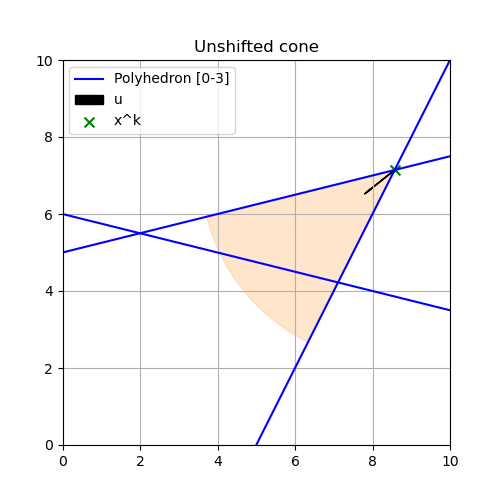
\includegraphics[width=200px]{images/unshifted_cone.png}
    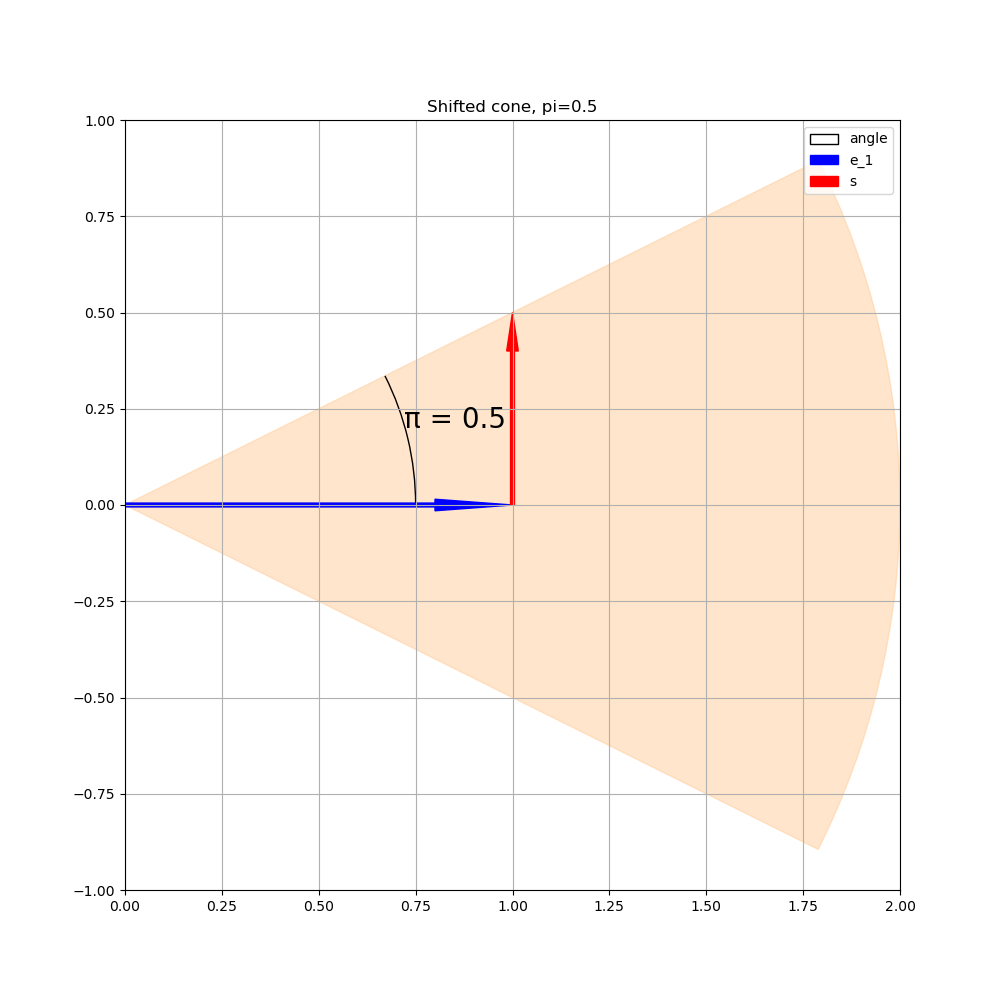
\includegraphics[width=200px]{images/shifted_cone.png}
    \caption[An example of the shifted and unshifted cones]
	{
		On the left is an unshifted cone $\unshiftedcone$.
		The polyhedra is in blue, and the current iterate in green.
		A feasible direction $u$ from the current iterate is calculated, and the width of the cone is determined to lie within the active constraints of the polyhedra.
		On the right is a shifted cone $\unshiftedcone$.
		It is centered at the origin, and points along $e_1$, opening at a rate of $\alphak$.
    }
    \label{linear_cones_images}
\end{figure}

Observe that, by construction, $\unshiftedcone$ is feasible with respect to the active constraints.
That is,  for all $x \in \unshiftedcone$,  and $i \in \activei\left(\xk\right)$, $\lca x \le \lcb_i$.
\cref{linear_cones_images} contains a depiction of these cones.


% = \left\{x \in \Rn \bigg | \quad x = \xk + t \uk+ s, s^Tu^{\star} = 0, t \ge 0, \|s\| \le {\alphak} t\right\}  \\
% \left\{x = (t, s)^T \in \Rn, t \in \mathbb R_{\ge 0}, s \in \mathbb R^{n-1} \bigg |\quad \|s\| \le {\alphak} t \right\} 

\begin{lemma}
\label[lemma]{unshiftedconeisfeasible}
Let $\unshiftedcone$ and $\polyk$ be defined by \cref{defineunshiftedcone} and \cref{polyhedron_k}.

The set $\unshiftedcone$ is feasible with respect to the active constraints of $\polyk$ at $\xk$.
\end{lemma}

\begin{proof}
Note that the trust region boundary cannot be active at $\xk$ as $\dk > 0$.
Let $\activei$, $\alphak$, and $\uk$ be defined by \cref{define_activei}, \cref{define_alpha_k}, \cref{define_u_k} and
$\lca$ and $\lcb$ be defined by \cref{eq:DFO-linear}.
Let $y = \xk + t\uk + s \in \unshiftedcone$ and $i \in \activei\left(\xk\right)$ be arbitrary.
Then,
\begin{align*}
{\lca}_{i}^Ty - {\lcb}_{i} = {\lca}_{i}^T(t\uk + s) = {\lca}_{i}^Ts + t {\lca}_{i}^T\uk \le \|s\| - \alphak t \le 0.
\end{align*}
\end{proof}

The following function is useful for showing results about our ellipsoids:
\begin{align}
f_{e}(\pi, \delta, r; x) = (x - \delta e_1)^T
\begin{pmatrix}
1 & \boldsymbol0^T \\
\boldsymbol 0 & \pi^{-2} \boldsymbol I \\
\end{pmatrix}
(x - \delta e_1) - r. \label{define_ellipsoid_function}
\end{align}

\begin{lemma}
\label[lemma]{shifted_ellipsoid_in_cone}
Let $\shiftedcone, f_e, \alphak$ be defined as in \cref{defineshiftedcone}, \cref{define_ellipsoid_function}, \cref{define_alpha_k}.
Then, for all $\delta > 0$, the ellipsoid
\begin{align}
\left\{x \in \Rn \bigg | f_e\left(\alphak, \delta, \frac 1 2 \delta^2; x\right) \le 0 \right\} \subseteq \shiftedcone.
\end{align}
\end{lemma}

\begin{proof}
Suppose that $x \in \left\{x \in \Rn \bigg| f_e\left(\alphak, \delta, \frac 1 2 \delta^2; x\right) \le 0 \right\}$, 
and let $t = x^Te_1$, $s=x - t e_1$. 
Then
\begin{align*}
f_e(x) \le 0 \Longrightarrow 
(x - \delta e_1)^T\begin{pmatrix}
1 & \boldsymbol0^T \\
\boldsymbol 0 & \left(\alphak\right)^{-2} \boldsymbol I \\
\end{pmatrix}(x - \delta e_1) \le \frac 1 2 \delta^2  \\
\Longrightarrow (t - \delta)^2 + \frac {1} {\left(\alphak\right)^2} \|s\|^2 \le \frac 1 2 \delta^2 \\
\Longrightarrow \|s\|^2 \le \left(\alphak\right)^2 \left[\frac 1 2 \delta^2 - (t - \delta)^2\right] \\
= \left(\alphak\right)^2 \left[t^2 - 2(t - \frac 1 2 \delta)^2 \right] \le \left(\alphak\right)^2t^2
\Longrightarrow \|s\| \le \alphak t.
\end{align*}
Thus, $x \in\shiftedcone$.
\end{proof}


\begin{lemma}
\label[lemma]{linear_mapping_works}
Let $\rotk$, $T_k$, $\unshiftedcone$, $\shiftedcone$ be defined as in
\cref{define_r}, \cref{define_affine_mapping}, \cref{defineunshiftedcone}, \cref{defineshiftedcone}.
Then $T_k(\unshiftedcone) = \shiftedcone$.
% and $T_k^{-1}(\shiftedcone) = \unshiftedcone$
\end{lemma}

\begin{proof}
Observe that $\rotk e_1 = \uk$, $\rotk \uk = e_1$, $\det(\rotk) = 1$, and 
$\rotk \rotk ^T = \rotk ^T\rotk = I$.

Suppose that $x \in \unshiftedcone$.
Then there exists $t \ge 0$ and $s \in \Rn$ such that $x = \xk + t \uk+ s$ where $s^T \uk = 0$ and $\|s\| \le {\alphak} t$.
Then $T_k(x) = t\rotk\uk + \rotk s = te_1 + \rotk s$.
Observe that $(Rs)_1 = (\rotk s)^Te_1 = s^T\rotk^T(\rotk \uk) = s^T \uk = 0$.
Hence,
$T_k(x) = \begin{pmatrix}
t \\
\sigma
\end{pmatrix}$ where $\sigma \in \mathbb R ^ {n-1}$ satisfies $\|\sigma\| = \|s\| \le \alphak t$.
Thus, $T_k(x) \in \shiftedcone$.
Conversely, if $\begin{pmatrix}
t \\
\sigma
\end{pmatrix} \in \shiftedcone$, then let
$s = \rotk^T\begin{pmatrix}
0 \\
\sigma
\end{pmatrix}$
to see that
$x = T_k^{-1}\left(\begin{pmatrix}
t \\
\sigma
\end{pmatrix} \right)= \rotk^T\left(t e_1 + \begin{pmatrix}
0 \\
\sigma
\end{pmatrix}\right) = t \uk + s$ where 
$\|s\| = \|\sigma\| \le \alphak t$.
Hence $T_k^{-1}\left(\begin{pmatrix}
t \\
\sigma
\end{pmatrix}\right) \in \unshiftedcone$.
\end{proof}


\begin{lemma}
\label[lemma]{ellipsoid_fits}
Let $\activei$, $f_e$, $\deltaf$ $\alphak$, $\rotk$, $T_k$, and $\polyk$ be defined by
\cref{define_activei}, \cref{define_ellipsoid_function}, \cref{define_deltaf}, \cref{define_alpha_k}, \cref{define_r}, \cref{defineshiftedcone}, and \cref{polyhedron_k}
respectively.

For each iteration $k$, if $\activei\left(\xk\right) \ne \emptyset$, the ellipsoid
\begin{align}
\ellipsek = \left\{x \in \Rn \bigg | f_e\left(\alphak, \deltaf, \frac 1 2 \deltaf^2; T_k(x)\right) \le 0\right\} \label{definefeasibleellipsoid}
\end{align}
satisfies $\ellipsek \subseteq \polyk$.
\end{lemma}

\begin{proof}
Let $\alphakp$, $\rotk$, $\unshiftedcone$, and $\shiftedcone$ be defined by
\cref{define_alphakp}, \cref{define_r}, \cref{defineunshiftedcone}, and \cref{defineshiftedcone}
respectively.


% Let $L$ be the shortest distance from $\xk$ to any point on a non-active constraint. 
% Define $\alphakp = \sqrt{\left(1 + \left(\alphak\right)^2 \right) \left(1 + \frac 1 {\sqrt{2}}\right)}$, and let $\deltaf = \frac 1 {\alpha'} L$.
We see that if $x \in \ellipsek$,
then by \cref{shifted_ellipsoid_in_cone} we have that $T_k(x) = \begin{pmatrix}t\\ \sigma\end{pmatrix} \in \shiftedcone$ for some $\sigma \in \mathbb R^{n-1}$
with $\left\|\sigma\right\| \le \alphak$, and
\begin{align*}
(x - \deltaf e_1)^T\begin{pmatrix}
1 & \boldsymbol0^T \\
\boldsymbol 0 & \left(\alphak\right)^{-2} \boldsymbol I \\
\end{pmatrix}(x - \deltaf e_1) \le \frac 1 2 \deltaf^2 \\
\Longrightarrow (t - \deltaf)^2 \le (t - \deltaf)^2 + \frac {1} {\left(\alphak\right)^2} \|\sigma\|^2 \le \frac 1 2 \deltaf^2 \\
\Longrightarrow t \le \left(1 + \frac 1 {\sqrt{2}}\right) \deltaf
\end{align*}
so that 
\begin{align*}
\|x\|^2 = t^2 + \|\sigma\|^2 \le \left(1 + \left(\alphak\right)^2 \right) t^2 
\le \left(1 + \left(\alphak\right)^2 \right) \left(1 + \frac 1 {\sqrt{2}}\right)^2 \deltaf^2 
= \left(\alphakp\right)^2 \deltaf^2 \\
\Longrightarrow \|x\| \le \alphakp \deltaf \le \min_{i \in [m] \setminus \activei\left(\xk\right)} \left[{\lcb}_i - \left({\lca}_i\right)^T\xk\right].
\end{align*}
Thus, all points within $\ellipsek$ are closer than the nearest point of a non-active constraint.
Combine this with \cref{unshiftedconeisfeasible} to see that $\ellipsek \subseteq \polyk$.
\end{proof}



\begin{lemma}
\label[lemma]{ellipsoid_includes_origin}
Let $\deltaf$, $\rotk$, $T_k$, $\unshiftedcone$, $\shiftedcone$, $\polyk$ be defined as in
\cref{define_deltaf}, \cref{define_r}, \cref{define_affine_mapping}, \cref{defineunshiftedcone}, \cref{defineshiftedcone}, \cref{polyhedron_k}.

For any iteration $k$,
the ellipsoid
\begin{align}
\scaledellipsek  = \left\{x \in \Rn | f_e\left({\alphak}, \sdk, \sdk^2; T_k(x)\right) \le 0\right\} \label{definescaledfeasibleellipsoid}
\end{align}
satisfies $\xk \in \scaledellipsek$.
\end{lemma}

\begin{proof}
We have that
\begin{align*}
f_e\left(\alphak, \deltaf, \deltaf^2; T_k\left(\xk\right) \right) =  
f_e\left({\alphak}, \deltaf, \deltaf^2; 0\right) = \\
(0 - \deltaf e_1)^T\begin{pmatrix}
1 & \boldsymbol0^T \\
\boldsymbol 0 & \left(\alphak\right)^{-2} \boldsymbol I \\
\end{pmatrix}(0 - \deltaf e_1) = \deltaf^2 \le \deltaf^2.
\end{align*}
\end{proof}








% 
% 
% 
% 
% We will first define the ellipsoid and show some of its properties within the transformed space $C_2$ before mapping it to $C_1$.
% To this end, fix an arbitrary $\delta > 0$ and let 
% $f_{e}(x): \Rn \to \reals $ be defined by 
% \begin{align}
% f_{e}(x) = (x - \delta e_1)^T\begin{pmatrix}
% 1 & \boldsymbol0^T \\
% \boldsymbol 0 & \alpha^{-2} \boldsymbol I \\
% \end{pmatrix}(x - \delta e_1) - \frac 1 2 \delta^2
% \label{define_ellipsoid_function}
% \end{align} 
% and consider the ellipsoid $E_1 = \{x | f_{e}(x) \le 0\}$.
% We will show that $E_1 \subseteq C_2$.
% To this end, suppose $x = (t, s) \in E_1$.
% Firstly, note that
% \begin{align*}
% 2\big(t - \frac {\delta} 2\big)^2 \ge 0
% \Longrightarrow 2t\delta - \frac 1 2 \delta^2 \le 2t^2 
% \Longrightarrow \frac 1 2 \delta^2 - (t - \delta)^2 \le t^2. 
% \end{align*}
% \Longrightarrow \frac 1 2 \delta^2 -t^2  + 2t\delta - \delta^2 \le t^2 \\
% \Longrightarrow 0 \le t^2 - t\delta + \frac 1 4 \delta^2
%  \Longrightarrow 0 \le 2t^2 - 2t\delta + \frac 1 2 \delta^2\\

% We choose this mapping because if $x = x_0 + t u^{\star} + s \in C_1$,
% then $\|s\|\le \alpha t \Leftrightarrow \|Rs\| \le \alpha t$ and $0 = s^Tu^{\star} = s^T R^T R u^{\star} = (Rs)^T e_1$ imply that 
% $R(x - x_0 - \delta u^{\star}) = t Ru^{\star} + Rs = t e_1 + Rs \in C_2$.
% Thus, the affine mapping $T : \Rn \to \Rn$ defined by $T(x) = R(x - x_0 - \delta u^{\star})$ maps $C_1$ to $C_2$.
% Conversely, the same arguments show that $T^{-1}(x) = R^Tx + x_0 + \delta u^{\star}$ maps $C_2$ to $C_1$.

%  \in SO(n)
% u = [3957; 6294.9]
% u = u / norm(u)
% e = [1; 0.0]
% a = e + u
% r = 2 * a * a' / (a' * a) - eye(2)
% r * e
% r * u


% 
% Having proven that $E_1 \subseteq C_2$, it follows that $T^{-1}(E_1) \subseteq C_2$.
% However, $T^{-1}(E_1) = \{ x \in \Rn | (x - \delta u^{\star})^TQ(x-\delta u^{\star} \le \frac 1 2 \epsilon\}$ where

% 
% \begin{align*}
% E_2 = \bigg \{x \bigg | (x - x_0 - \delta u^{\star})^T\bigg(R^T\begin{pmatrix}
% 1 & \boldsymbol0^T \\
% \boldsymbol 0 & \alpha^{-2} \boldsymbol I \\
% \end{pmatrix}R\bigg)(x - x_0 - \delta u^{\star}) \le \frac 1 2 \delta^2 \bigg\}.
% \end{align*}
% We know that $x \in E_1 \Leftrightarrow T(x) = R(x - x_0 - \delta u^{\star}) \in E_2 \Longrightarrow T(x) \in C_2 \Longrightarrow x = T^{-1}\left(T(x)\right) \in C_1$.
% Thus, we know that the ellipsoid $E_2$ is contained within the active constraints, and can be scaled by $2$ to include $x_0$.

\begin{lemma}
\label[lemma]{nontrivial_ellipsoid_exists}
Let $\activei$ and ${\alphak}$ be defined by \cref{define_activei} and \cref{define_alpha_k} respectively.

Suppose that \cref{interior_point} holds.

For some iteration $k$, if $\activei \ne \emptyset$, then the ellipsoid defined by \cref{define_linear_nontrival_ellipsoid}
is suitable according to definition \cref{define_suitable_ellipsoid}.

% For iteration $k$, if ${\alphak} > 0$, then there exists a suitable ellipsoid for iteration $k$ according to .
\end{lemma}

\begin{proof}
Let 
$f_e$,
$T_k$,
$\rotk$, $\deltaf$, and $\scaledunshiftedellipsoid$
be defined as in
\cref{define_ellipsoid_function},
\cref{define_affine_mapping},
\cref{define_r},
\cref{definefeasibleellipsoid}, and
\cref{definescaledfeasibleellipsoid}
respectively. 
Observe \cref{define_suitable_ellipsoid} with \cref{define_linear_nontrival_ellipsoid} defines  $\ellipsek$ and $\scaledellipsek$ to be
\begin{align*}
\begin{array}{cccc}
\ellipsek &=& \left\{x \in \Rn \bigg | f_e\left(\alphak, \sdk, \frac 1 2 \sdk^2; T_k(x)\right) \le 0\right\}, &\quad \textrm{and}  \\
\scaledellipsek &=& \left\{x \in \Rn \bigg | f_e\left({\alphak}, \sdk, \sdk^2; T_k(x)\right) \le 0\right\}.&
\end{array}
\end{align*}

By \cref{ellipsoid_fits}, we know that $\ellipsek \subseteq \polyk$.
By \cref{ellipsoid_includes_origin}, we know that $\xk \in \scaledellipsek$ .
By \cref{alphas_are_bounded}, there exists $\epsilon_{\alpha} > 0$, such that the condition number 
$\condition\left(\qk\right) = \frac{\max\{1, {\alphak}^{-2}\}}{\min\{1, {\alphak}^{-2}\}} = {\alphak}^{-2} > 0$.
This is because $\det\left(\rotk\right) = 1$ means the condition number of $\qk$ is not affected $\rotk$.
\end{proof}


% Let
% \begin{align*}
% \qk = \rotk^T\begin{pmatrix}
% 1 & \boldsymbol0^T \\
% \boldsymbol 0 & {\alphak}^{-2} \boldsymbol I \\
% \end{pmatrix}\rotk \\
% c_k = \xk - \deltaf \uk \\
% \epsilon = \delta^2 
% \end{align*}


%
%\begin{boxedcomment}
%I think we no longer use this result...
%\end{boxedcomment}
%
%\color{red}
%We use the following result shown \cite{BillupsLarson2013}, Corollary 4.7.
%We restate the theorem here, with the simplication that $f$ is deterministic function:
%
%\begin{assumption}
%\label{fully_quadratic_assumption}
%Suppose that a set $S$ and a radius $\dmax$ are given.
%Assume that $f$ is twice continuously differentiable with Lipshcitz continuous Hessian in an open domain containing the $\dmax$ neighborhood
%$\cup_{x \in S} B(x; \dmax)$ of the set $S$.
%\end{assumption}
%
%\begin{lemma}
%\label[lemma]{larson_change_radius} 
%Let $Y$ be a poised set of $p$ points, and let $R = \max_{i}\|y^i - y^0\|$.
%Let $f$ satisfy \cref{fully_quadratic_assumption} over some convex set $\Omega$, and let $m(x)$ denote the quadratic model of $f$ using \cref{reg}.
%If $f$ is a Lipschitz continuous function with Lipschitz constant $L_g$, and $m_f(x)$ is a quadratic model of $f$.
%Then, there exist constrants $\Lambda_1, \Lambda_2, \Lambda_3$ independent of $R$ such that for all $x \in B(y^0, R)$,
%\begin{align*}
%\|f(x) - m_f(x)\| \le 4\Lambda_1 R^3L \sqrt{p+1} \\
%\|\nabla f(x) - \nabla m(x)\| \le 4\Lambda_2R^2  L \sqrt{p+1} \\
%\|\nabla^2 f(x) - \nabla^2 m(x)\| \le 4\Lambda_3  RL \sqrt{p+1}
%\end{align*}
%\end{lemma}
%
%\color{black}

% 
% \sbnote{There needs to be some discussion about how the method defined above to construct the suitable ellipsoid relates to the other methods 
% you described}.

\subsection{Ellipsoid Searches}

Within \cref{the_safe_ellipsoid}, we showed how to construct one possible ellipsoid that satisfies \cref{define_suitable_ellipsoid}.
In practice, this ellipsoid could be less than desirable.
Within this section, we discuss the requirements of other variants of the \emph{ConstructTrustRegion} subroutine that we explored for practicality.
The key requirement is these ellipsoids must still satisfy \cref{define_suitable_ellipsoid} to share the same convergence results.

\subsubsection{Ensuring Suitability}

To retain the convergence results, these algorithms maintain $\ellipsek \subseteq \polyk$,
$\xk \in \scaledellipsek $, and a bound on $\condition\left(\qk\right)$.

To ensure the condition number is bounded, the algorithm can compute the condition number of the safe ellipsoid, and only consider ellipsoids better conditioned.
Alternatively, it could introduce its own bound.
We found it simplest to parameterize ellipsoids by their Cholesky factorization $\qk = LL^T$.
Namely, we parameterized the search space in terms of a lower triangular matrix $L$, and required the diagonal entries to be positive.
To ensure a bounded condition number, we constrain  $\max_{i\in[n]} \le \epsilon_{\alpha} \min_{i \in [n]}$.
Then requiring a 

One potential difficulty created by moving the ellipsoid center $\ck$ is that the current iterate $\xk$ may not lie within near the resulting ellipsoid.   
The pitfall is that the model function may lose accuracy near the current iterate.
Thus, we have implemented a few ways of ensuring the current iterate is within the search trust region.
This can be done by either of the following two options:
\begin{itemize}
\item Adding a constraint to the ellipsoid problem to include the original point.
\item Expand the size of the ellipsoid.
\end{itemize}

\paragraph*{Adding a constraint.}
In order to include the original point as a constraint, we add a constraint of the following form to the definition of the ellipsoid.
\begin{align*}
\frac 1 2 \left(\xk - \ck\right)^T\qk\left(\xk - \ck\right) \le \frac 1 2 \sdk^2.
\end{align*}
Constraints of this nature make finding the ellipsoid much more expensive:
the optimization problem we construct uses ${\qk}^{-1}$ as decision variables, so that constraints in terms of $\qk$ must model matrix inversion.

\paragraph*{Increase the radius.}
An alternative is to scale $\qk$ by a constant.
We use the scaling factor $\sdk$ defined by
\begin{align*}
\sdk = \max \left\{1, \sqrt{\left(\xk - \ck \right)^T \qk \left(\xk - \ck \right)} \right\}
\end{align*}
and let the ellipsoid be:
\begin{align*}
\ellipsek = \left\{x \in \Rn \bigg| \frac 1 2 \left(x - \ck\right)^T \qk \left(x - \ck\right) \le \frac 1 2 \sdk^2\right\}.
\end{align*}
However, this means that in general $\ellipsek \not \subset \feasible$.
so that the sample points must be contained to also lie within the feasible region: $\ellipsek \cap \feasiblek$.
For details on how to choose sample points with additional constraints, see \cref{model_improving_algorithm}.


 \sbnote{This raises a number of questions.
 First is whether the current iterate will be a sample point.
 If it isn't, then the model function may disagree with the true function at the current iterate, 
 so descent of the model function may not correspond to descent of the true function, even for very small steps.
 Also, if the search region is chosen to be equal to the ellipsoidal region, then we may not be able to get descent at all.
 At the end of the day,  we don't necessarily need the current iterate to be in the ellipsoid as long as
 1) it is within the search trust region, and 2) the model function is sufficiently accurate over the search trust region.
 Actually, we don't even need 2), do we?  We just need the accuracy condition to be satisfied at the current iterate, right?}


\subsubsection{Maximal Volume}
\label{ellipse_optimization}
The error bounds given in \cref{shifted_ellipsoid} suggest that we can obtain more accurate model functions by 
minimizing the condition number of the matrix $\qk$.
However, we also desire a large ellipsoid so that our model will satisfy the error bounds over more of $\searchtrk$.
Thus, one choice for $\sampletrk$ is to choose the maximum volume ellipsoid that is both feasible and lies within the outer trust region.
We can accomplish this for various ellipsoid centers, by finding the maximal volume ellipsoid that is constrained to lie within the polytope
$\polyk := \left\{x \in \Rn | \lca x\le \lcb,   \xki - \dk \le x_i \le \xki + \dk\right\}.$
% Note that we have replaced the usual trust region $B_2\left(\xk, \dk\right)$ with an $L_{\infty}$ ball, called the {\em outer trust region},
% defined in \cref{define_outer_trust_region}.

This is not the only reasonable approach: maximizing ensures a larger region for which the models will be accurate, 
but we are most interested in decent directions.
Namely, we may wish to use previously evaluated points to provide a hint where the next ellipsoid should be.
Another consideration is where points have been evaluated: it may be more economical to choose a smaller ellipsoid that can reuse existing points.
However, in this section,  we consider the problem of choosing $\qk$ and $\sdk$ to maximize the volume of $\ellipsek \subseteq \polyk$ given a fixed center $\ck$.
Later, in \cref{center_searches}, we will explore strategies for moving the center of the ellipsoid in order to improve performance of our trust region algorithm.

We adopt a method similar to that described in \cite{Khachiyan1993},
which presents an algorithm for finding the maximum volume inscribed ellipsoid for a polytope.
% For the remainder of this section, we drop the superscript $(k)$ and write
% \begin{align*}
% P = \polyk =  \{ x \in \Rn\; | \;  Ax \le b \}.
% \end{align*}
% We wish to find the maximum-volume ellipsoid $E \subseteq P$ centered at a point $c \in P$.

% \bar{\lctrb}
Let $\bar g = \lctrb - \lctra \ck$ and $d = x - \ck$ so that the polytope becomes
\begin{align*}
\polyk = \left\{ \ck + d \in \Rn \; | \;  \lctra d \le \bar{g} \right\}
\end{align*}
Using this transformation, the ellipsoid can then be centered at zero, and defined by a symmetric positive definite matrix $Q \succ 0$:
\begin{align*}
E = \left\{ d \in \Rn \; \bigg | \; \frac 1 2 d^T Q d \le 1 \right\}.
\end{align*}
Our goal is to determine the matrix $Q$ that maximizes the volume of $E$ such that $\mu + E \subset P$.
This is accomplished by solving the following problem for $Q$ for a given center:
 \begin{align}
\begin{array}{cc}
 \sup_{Q \succeq 0} & \det(Q^{-1})  \\
 \textrm{s.t.} & A_i^T Q^{-1} A_i \le \frac 1 2 \bar{b_i}^2.
\end{array}
 \label{ellipse_1}
\end{align}


\begin{theorem} 
Let $\mathcal{P} = \{x \in \Rn | Ax \le b\}$, 
where $A$ is an $m \times n$ matrix, 
and $b \in \Rm$.  Let $c \in \intr{P}$.

Suppose that $Q$ solves \cref{ellipse_1}, where $\bar{b} = b - Ac$.
Then the ellipsoid $E = \{ x \in \reals^n | (x-c)^T Q(x-c) \le 1\}$ has the maximum volume over all ellipsoids centered at $c$ and contained in $P$.
\end{theorem}

\begin{proof}
Define the auxiliary function $f(d) = \frac 1 2 d^T Q d$ so that $E = \{ d \in \Rn\; | \; f(d) \le 1 \}$.
Because $Q$ is positive definite, $f$ has a unique minimum on each hyperplane $A_i d = b_i$.
Let this minimum be $d^{(i)} = \argmin_{A_id =\bar{b}_i} f(d)$ for $i\in[m]$.
By the first-order optimality conditions, there exists a $\lambda \in \Rm$ such that for each $i\in[m]$,
\begin{align*}
\nabla f(d^{(i)}) = Q d^{(i)} = \lambda_i A_i.
\end{align*}
Since $A$ is invertible, we have $d^{(i)} = \lambda_i Q^{-1}A_i$. 
We also know that $A_i^T d^{(i)} = \bar{b_i}$, so 
\begin{align*}
A_i^T \lambda_i Q^{-1}A_i = \bar{b_i} \Longrightarrow
\lambda_i = \frac {\bar{b_i}}{A_i^T  Q^{-1}A_i},
\end{align*}
so that
\begin{align*}
d^{(i)} = \lambda_i Q^{-1}A_i = \frac {\bar{b_i}}{A_i^T  Q^{-1}A_i}  Q^{-1}A_i \quad \forall 1\le i\le m.
\end{align*}

Because $E \subset P$, we also know that $f(d^{(i)}) \ge 1$ for each $i$. Thus,
\begin{align*}
\frac 1 2 (d^{(i)})^{T} Q d^{(i)} \ge 1 \\
\Longrightarrow & \frac 1 2 \bigg(\frac {\bar{b}_i}{A_i^T  Q^{-1}A_i}  Q^{-1}A_i\bigg)^{T} Q \frac {\bar{b}_i}{A_i^T  Q^{-1}A_i}  Q^{-1}A_i \ge 1 \\
\Longrightarrow & \frac 1 2 \frac {1}{A_i^T  Q^{-1}A_i}  \bar{b_i} A_i^T Q^{-1} Q \frac {\bar{b_i}}{A_i^T  Q^{-1}A_i}  Q^{-1}A_i \ge 1 \\
\Longrightarrow & \frac 1 2 \frac {1}{A_i^T  Q^{-1}A_i}  \frac {\bar{b_i}^2}{A_i^T  Q^{-1}A_i}  A_i^T Q^{-1}A_i \ge 1 \\
\Longrightarrow & \frac 1 2  \frac {\bar{b_i}^2}{A_i^T  Q^{-1}A_i} \ge 1 \\
\Longrightarrow & \frac 1 2 \bar{b_i}^2\ge A_i^T  Q^{-1}A_i \\
\Longrightarrow & A_i^T  Q^{-1}A_i \le \frac 1 2 \bar{b_i}^2
\end{align*}

Because the volume of the ellipsoid is proportional to the determinant of $Q^{-1}$, the maximal ellipsoid is defined by \cref{ellipse_1}.
\end{proof}


Notice that the constraints for \cref{ellipse_1} can be simplified for the outer trust region's constraints.
These take the form:
\begin{align*}
e_i^T\left(\frac{\qk}{\frac 1 2 \sdk^2}\right)^{-1} e_i \le \left[e_i^T\left(\xk - \ck\right) \pm \dk \right]^2 \quad \forall i \in [n]
\end{align*}
or
\begin{align}
\label{ellipsoids_trust_region_constraints}
\left(\frac{\qk}{\frac 1 2 \sdk^2}\right)_{i,i}^{-1} \le \left[\xki - \ck_i \pm \dk \right]^2 \quad \forall i \in [n].
\end{align}


\section{Polyhedral Trust Region Approach}
\label{sec:polyhedral}

One simple approach to ensuring that all sample points are feasible is to restrict them to lie within the intersection of the feasible region and the outer trust region.
In particular,  we define the sample and search trust regions by
\[ \sampletrk = \searchtrk = \feasible \cap \outertrk.\]
Note that by using an $L_{\infty}$-ball for the outer trust region, both $\sampletrk$ and $\searchtrk$ are polytopes.
 
The main challenge in implementing this approach is ensuring that the sample points chosen from within $\sampletrk$ are well-poised.
To accomplish this, we modify the model improvement algorithm given by \cref{model_improving_algorithm}.   
Recall that \cref{model_improving_algorithm} works on a shifted and scaled problem in which sample points are selected to lie within a unit ball.
Thus,  in Step 2 of that algorithm,  each new sample point $\hat{y}$  is selected by  
$\hat{y} \in \argmax_{t:\norm{t} \le 1} \left|u_i(t)\right|$, where the pivot polynomials $u_i$ are constructed during the algorithm.  
We modify this step by choosing $\hat{y} \in \argmax_{t\in \sampletrk} \left|u_i(t)\right|$.  



%That is, we add the constraints $\mcik(x) \le 0 \forall i \in \mathcal{I}$ and $\mcik(x) = 0 \forall i \in \mathcal{E}$ to the model improvement algorithm while selecting new points.
%This constrains the new points to also lie within the current model of the trust region in \cref{model_improving_algorithm}, Step 2.
%The search space for this optimization problem will be the feasible region intersect the trust region: $\feasible \cap \outertrk $.

The challenge lies in finding sufficiently poised sample points.
Note that \cref{model_improving_algorithm} uses a parameter $  \ximin $ as a lower bound of the pivot values of the Vandermonde matrix.
For unconstrained problems, this approach could always find a pivot value for any $ \ximin \in (0,1)$ because it optimized over a sphere.
However, when requiring points to live within $ \feasible \cap \outertrk $, it can happen that even after replacing a point, we still have not satisfied this bound.
In \cref{lspc}, for some values of $  \ximin $, there is no point in $ \feasible \cap \outertrk $ that will leave a sufficiently large pivot.

\begin{figure}[ht]
    \centering
    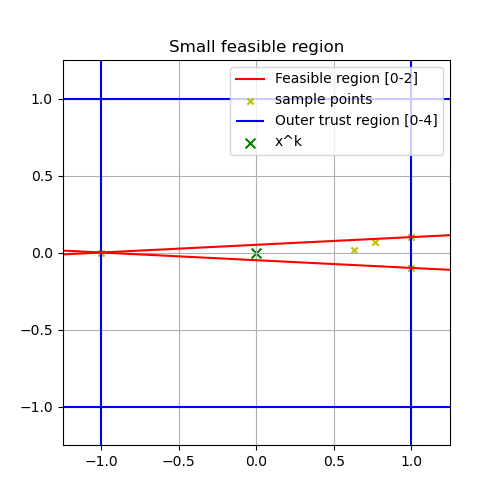
\includegraphics[width=200px]{images/small_sample_region.png}
    \caption[An example of constraints limiting sample point choices.]
    	{An example of constraints limiting sample point choices.
    	If the constraints remove a large region of the trust region, there may be no feasible $\Lambda$-poised set.
    }
    \label{lspc}
\end{figure}

%As the number of dimensions grows the ratio of volume of the trust region intersect the feasible region to the feasible region can become smaller.

One way to handle this is to  introduce a $\xi_{\text{cur}}$ which is allowed to decrease.
(Possibly, until a threshold is reached for maintaining a fixed $\Lambda$.)
If the new point does not improve the geometry of the set significantly, then there is no other point that would do better.
To test this, we introduce a constant $\delta_{\text{improv}}>0$ and require a new point to increase the current pivot by a factor greater than $\delta_{\text{improv}}$.
If the new point does not satisfy this test, we proceed with our current point and possibly decrease $\xi_{\text{cur}}$.
Conceptually, 
\begin{itemize}
\item $\ximin$ is a tolerance that ensures Step 3 does not perform division by zero,
\item $\xi_{\text{cur}}$ measures the most poised set possible within $\sampletrk$,
\item and replacement points are ignored if they do not improve the poisedness by more than $\delta_{\text{improv}}$.
\end{itemize}
The new modified improvement algorithm is described in \cref{modified_model_improving_algorithm}.
The \emph{ConstructTrustRegion} subroutine for this approach follows the prototype with $\sampletrk = \searchtrk = \feasible \cap \outertrk $.
As usual, we may also wish to remove points larger than a certain radius from the current model center.

\begin{algorithm}[H]
    \caption{Modified Model Improvement Algorithm}
    \label{modified_model_improving_algorithm}
    \begin{itemize}
        \item[\textbf{Step 0}] \textbf{(Initialization)} \\
            Given an interpolation set $\sampletrk$, and set $Y$ of $p+1$ points,
            initialize $i=1$, $0 < \ximin < \xi_{\text{desired}}$, $0 <\delta_{\text{improv}} < 1$,
            $  \xi_{\text{cur}} = \xi_{\text{desired}}$.
            
		\item[\textbf{Step 1}] \textbf{(Pivot)} \\
			Compute the next pivot index $j^{\textrm{max}}_i = \argmax_{i \le j \le |Y|-1} \left|u_i\left(y^j\right)\right|$,
			and swap points $i$ and $j^{\textrm{max}}_i$ within $Y$.
			
        \item[\textbf{Step 2}] \textbf{(Check threshold)}
                If $\left|u_i\left(y^i\right)\right| \ge \xi_{\text{cur}}$ then go to Step 3. \\
                Compute $ \hat y = \arg\max_{t \in \sampletrk \cap \feasible}\left|u_i(x)\right|$ \\
                If $ |u_i(\hat y)| < \ximin$ then \textbf{Stop}: the algorithm failed \\
                If $|u_i(\hat y)| - \xi_{\text{cur}} \ge \delta_{\text{improv}} \xi_{\text{cur}}$ then
                replace point $y^i$ with $\hat y$ and set $\xi_{\text{cur}} \gets |\phi_i(\hat y)|$
                
        \item[\textbf{Step 3}] \textbf{(Gaussian elimination)} \\
        	For $j = i+1, \ldots, p$: \\
        	Set $u_j(x) \gets u_j(x) - \frac{u_j\left(y^i\right)}{u_i\left(y^i\right)} u_i(x)$ \\
            If $i = p$ then \textbf{Stop}, otherwise Set $i \gets i+1$ and go to Step 1
    \end{itemize}
\end{algorithm}

\paragraph*{Algorithm Conjecture}

When the algorithm fails, it is likely because $\sampletrk$ nearly contained in a subspace 
for which some basis function can be written as a linear combination of other basis functions.
Because our feasible region contains an interior point, we would expect that sufficiently small values of $\ximin>0$ allow the algorithm to run to completion.
However, for non-linear constraints, or even equality based constraints, there may not be such a $\ximin$.

Intuitively, higher order monomials would not improve the accuracy of the model over $\sampletrk$ 
if their function values do not significantly differ from that of a linear combination of lower order monomials.
This insight inspires a model improving algorithm that uses Gaussian elimination with {\em full pivoting}
to select only those monomials {\em useful} for approximating functions over $\sampletrk$.
When there is no replacement point or corresponding monomial in the basis that can be added to the existing set of Lagrange polynomials with a pivot larger than $\ximin$,
the algorithm would simply stop the Gaussian elimination.
Note that the maximization over $\sampletrk$ to find a replacement point would need to maximize $|u_j|$ for several $i \le j \le p$ rather than simply $i$.

% If a lower bound $\kappa_{\phi}$ on the maximum value of each polynomial is known ahead of time, then the check on \cref{impossibly_poised} is not needed.
% That is, for a given set of linear constraints and largest trust region radius, it may be possible to calculate $\xi_{\text{min}} \le \kappa_{\phi} \le \max_{V}\max_{j}\max_{i}\|\phi_i(y^j)\|$.
%Another interesting approach we have not investigated is to decrease the size of the sample set when a new point cannot be computed.
%The analysis for this approach may be more difficult.

\section{Results}

\subsection{Algorithm Variants}

\subsubsection{Circular Trust Region}
The simplest approach to maintaining a feasible trust region is to set the inner trust region radius sufficiently small.
Within the \emph{ConstructTrustRegion} subroutine, this method sets the trust region radius to the distance to the closest constraint:
$\outertrk = B_2\left(\xk, \min\left\{\dk, \min_{i}\frac{\left|A_i\xk - b_i\right|}{\left\|A_i\right\|} \right\}\right)$.
In practice, this does not work well as the radius can become too small to allow adequate progress.

Two general strategies were considered for addressing this issue as illustrated in \cref{options_basis}.
One option is to shift the center of the inner trust region as long as it remains within the outer trust region.
The second option is to elongate the trust region along the nearest constraint as discussed in the next section.
Of course, both of these can be done at the same time.


\begin{figure}[ht]
    \centering
    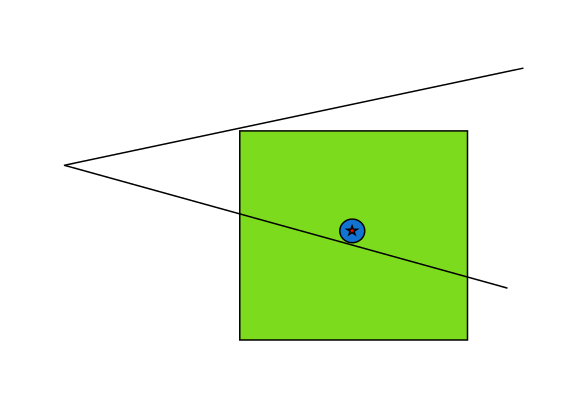
\includegraphics[width=200px]{images/small_circle.png}
    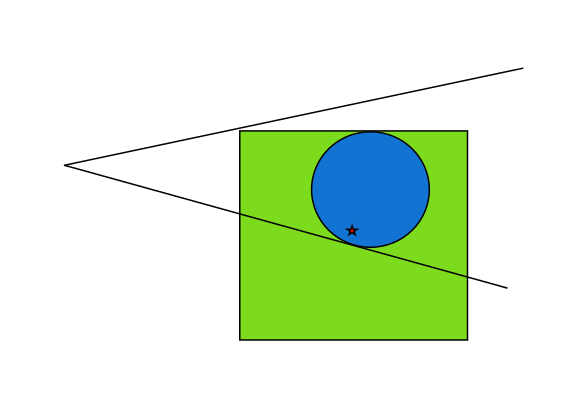
\includegraphics[width=200px]{images/shifted_center.png}
    \caption[The advantage of not requiring the sample region center to be the trust region center.]{
    	When the current iterate is too close to a constraint, the circular trust region becomes too small.
    	Shifting the trust region center helps remedy this.
    	The star is the current iterate, the green is the outer trust region, and blue the inner.
    }
    \label{options_basis}
\end{figure}


In order to address this issue we considered using ellipsoidal trust regions.
Whereas the circle does not allow improvement when the current iterate lies along a constraint, an ellipsoid elongates along this constraint.
In figure \cref{ellipse_adv}, we have this type of iterate, but by using an ellipsoid we are still able to search towards the vertex of the feasible region.
\begin{figure}[ht]
    \centering
    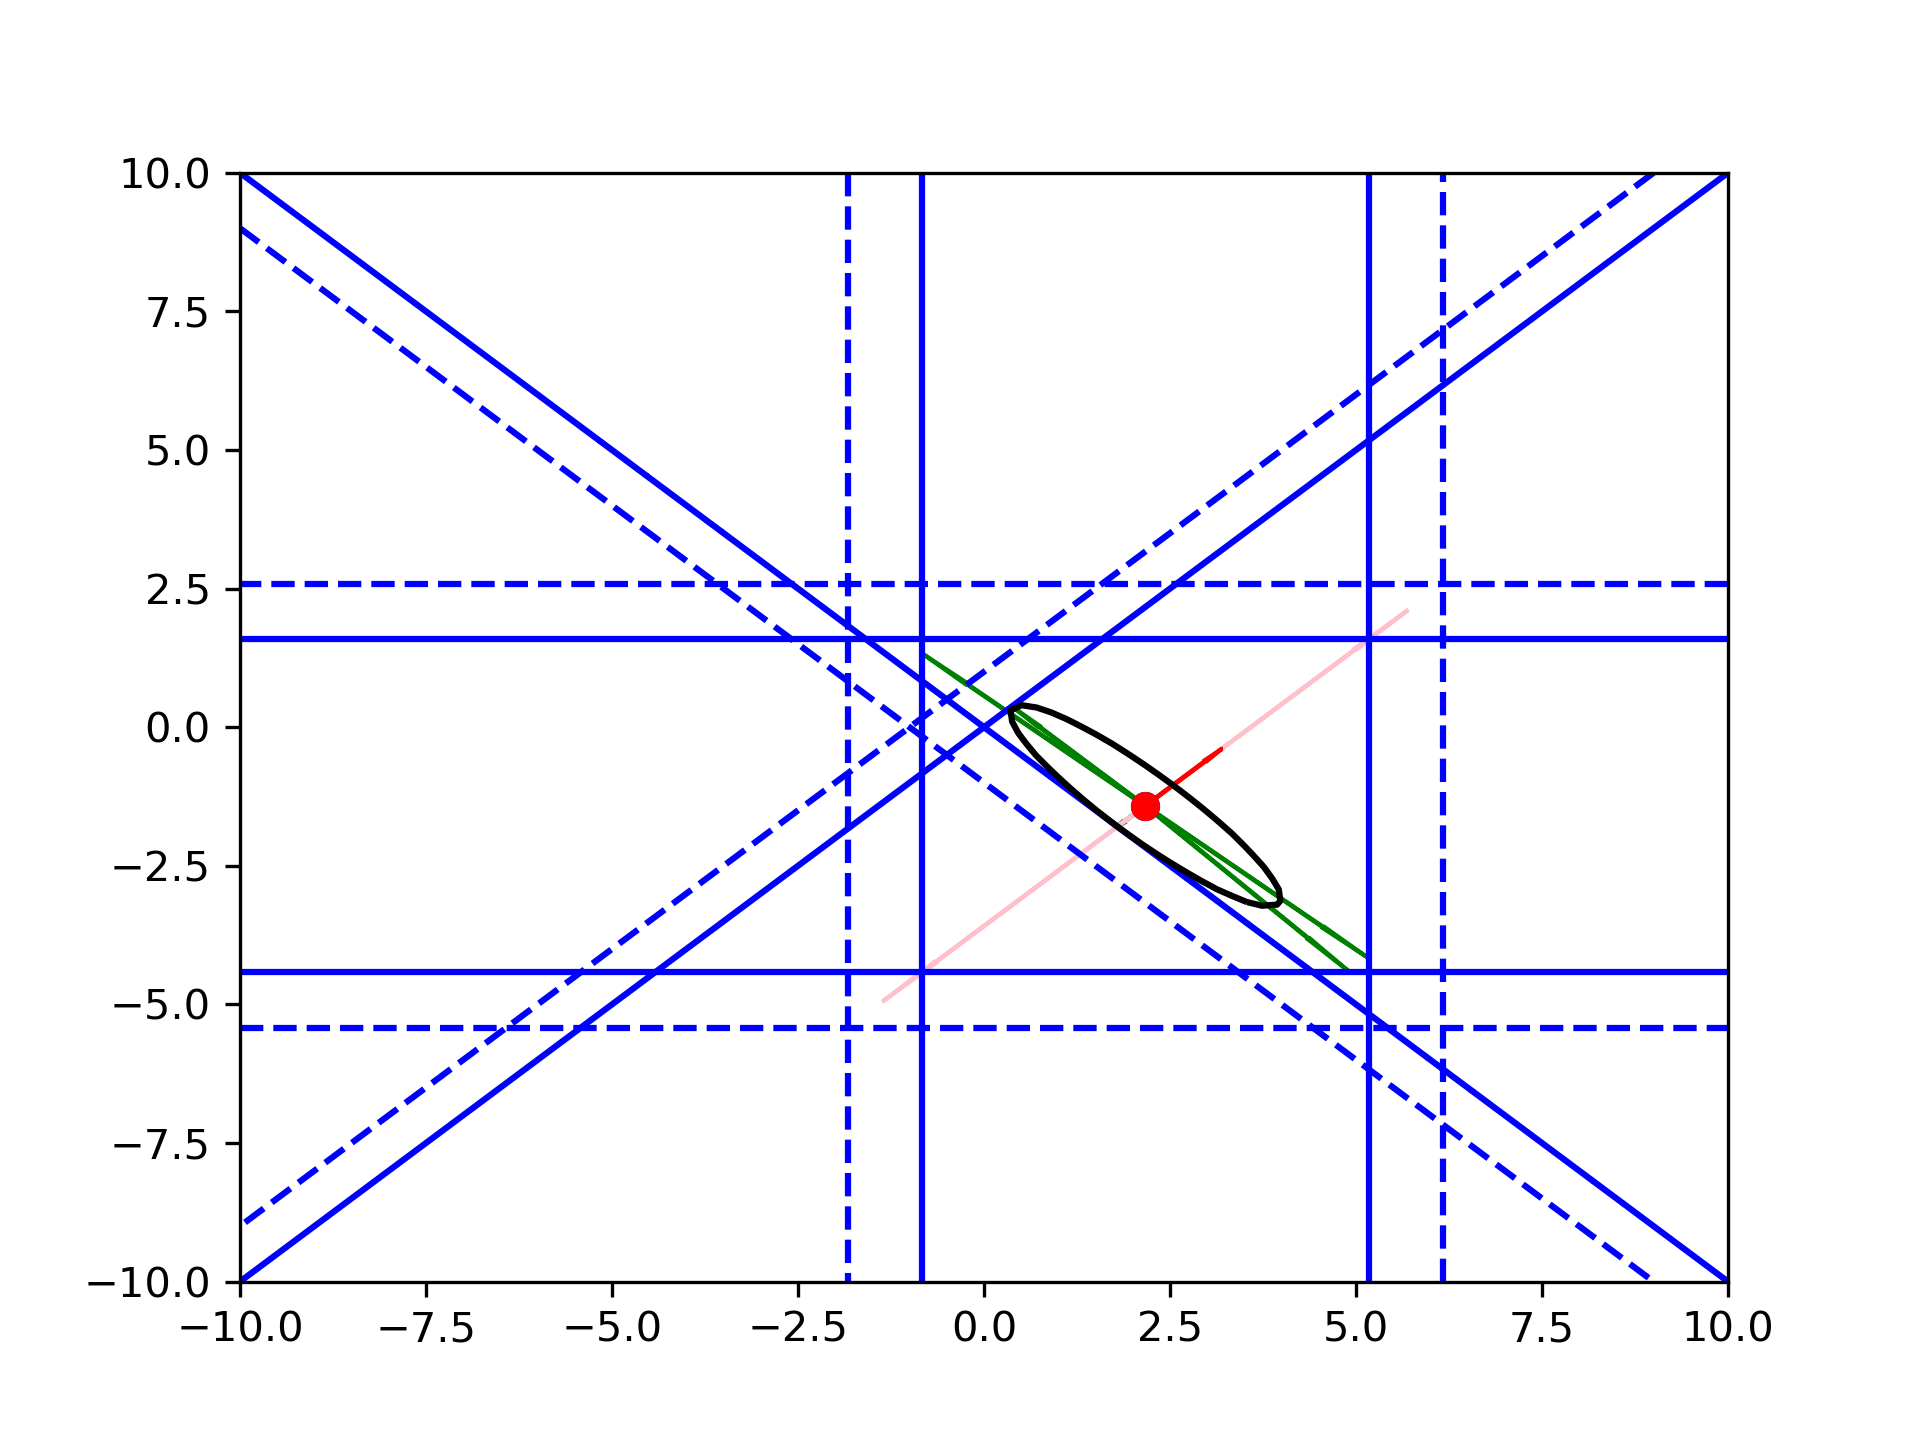
\includegraphics[scale=0.4]{images/advantage_of_ellipse_2.png}
    \caption[An ellipsoidal trust region allows for more progress than a circular trust region.] {
    	Although the center of the ellipsoid is close to the boundary of the constraints, it can elongate to allow progress.
    }
    \label{ellipse_adv}
\end{figure}


More specifically, at iteration $k$, we choose a scaling factor $\sdk$ and solve for an ellipsoid center $\ck \in \Rn$ and positive definite matrix $\qk$ to define an ellipsoid
\begin{align*}
\ellipsek = \left\{x \in \Rn \bigg| \; \frac 1 2 \left(x - \ck\right)^T\qk\left(x - \ck\right) \le \frac 1 2 \sdk^2 \right\}.
\end{align*}
The simplest approach is to simply let the center of the ellipsoid be the current iterate: $\ck = \xk$.





% \item How do we choose $\ellipsek$ to make the  ellipsoid as large as possible while ensuring that $ \ellipsek \subset \outertrk \cap \feasible $?




% ====================
% \sbnote{Move the following to somewhere else.}
% The advantage of the ellipsoidal trust region approach \cref{bluepill} is that we can reuse classical methods for ensuring good geometry.
% We can construct $\sampletrk$ to be ellipsoidal and use efficient algorithms within \cite{introduction_book} to satisfy \cref{accuracy}.
% However, we must be careful while choosing $ \searchtrk$ to allow sufficient reduction when we solve the trust region subproblem using the inner trust region.
% The search trust region is used while selecting the next iterate:
% \begin{align*}
% \sk = \argmin_{s \in \searchtrk} \mfk(\xk + s).
% \end{align*}
% =====================






\subsubsection{Choosing the Ellipsoid Center}
\label{center_searches}

The most obvious choice for the center of the ellipsoid is to choose $\ck$ (i.e., the current iterate).  
However, if $\xk$ is too close to a boundary of the feasible region, this can result in a badly shaped or very small ellipsoid.
We therefore explore strategies where the \emph{ConstructTrustRegion} subroutine moves the center of the ellipsoid away from the boundary. 
This is depicted in \cref{ellipse_adv}.


% We let the volume of the ellipsoid $E$ at center $c$ be given by $V(c) = \det(Q^{-1}) $.

\paragraph{Outer Trust Region Search}

One approach is to search all possible centers within $\feasible \cap \outertrk $.  
% That is, we solve:  \sbnote{Why do you use $\sdk$ in the following?}
% \begin{align*}
% \ck = \sup_{c \in \feasible \cap \outertrk} V(c)
% \end{align*}
% where $V(c)$ is the volume of the ellipsoid defined in \cref{ellipse_1}.

This has the advantage that it allows for the largest volume.
However, one problem with this search is that it can force the trust region away from the descent direction.
Notice that in \cref{ellipse_runs_away}, although the ellipsoid found has larger volume than before being shifted, 
this ellipsoid contains points farther from the corner that happens to contain the trust region's minimizer.
Within the results, these algorithms are described as ``ellipse everywhere''.

The following section addresses this problem by proposing a path search method for choosing the ellipsoid center.

\begin{figure}[ht]
    \centering
    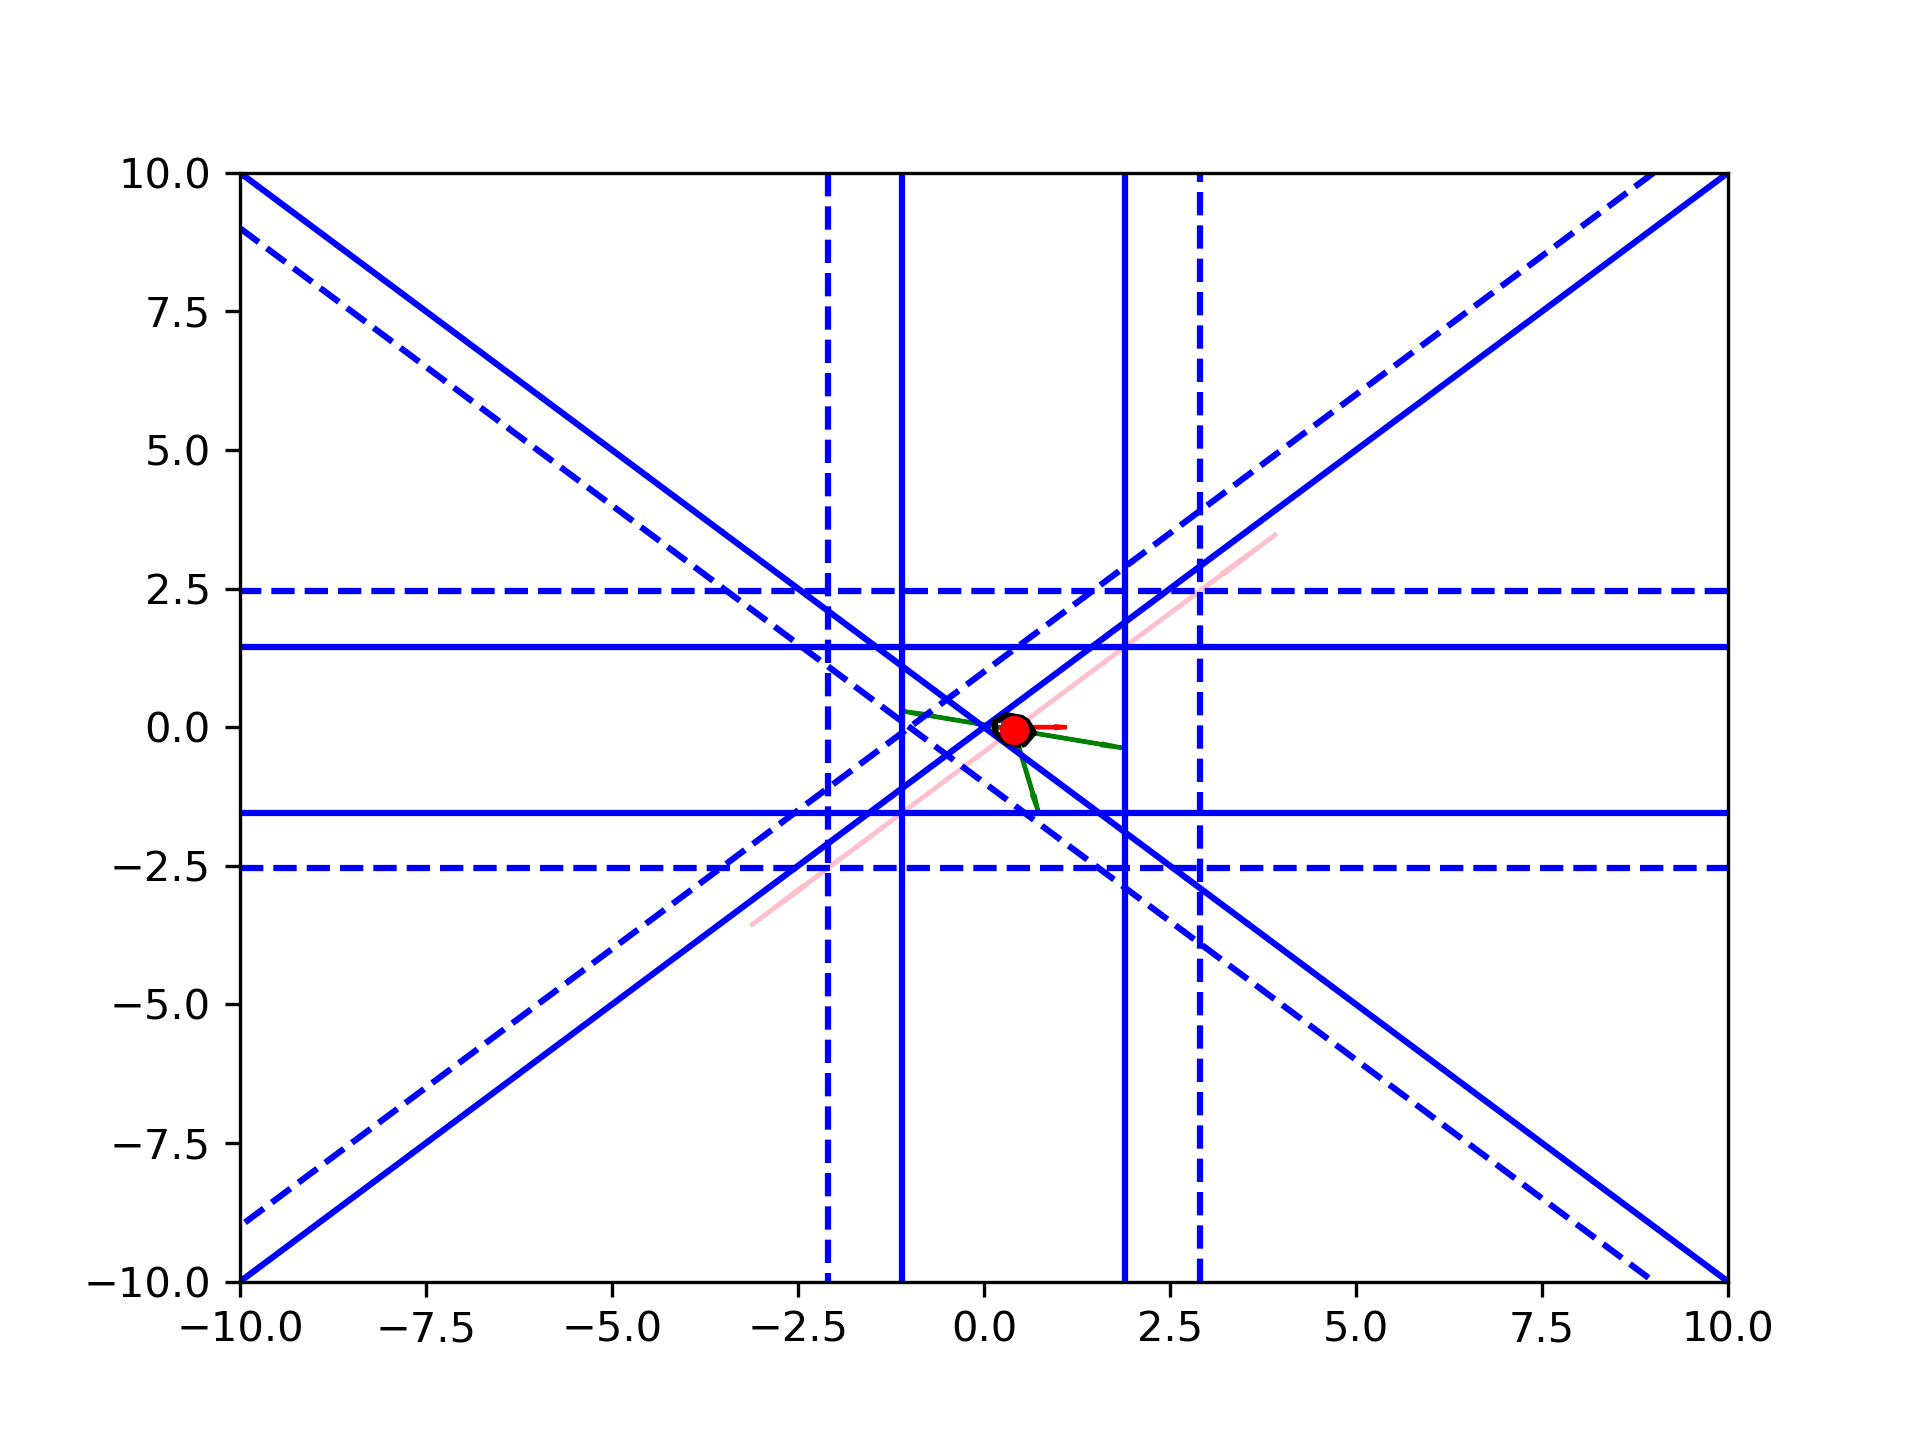
\includegraphics[scale=0.4]{images/everything_runs_1.png}
    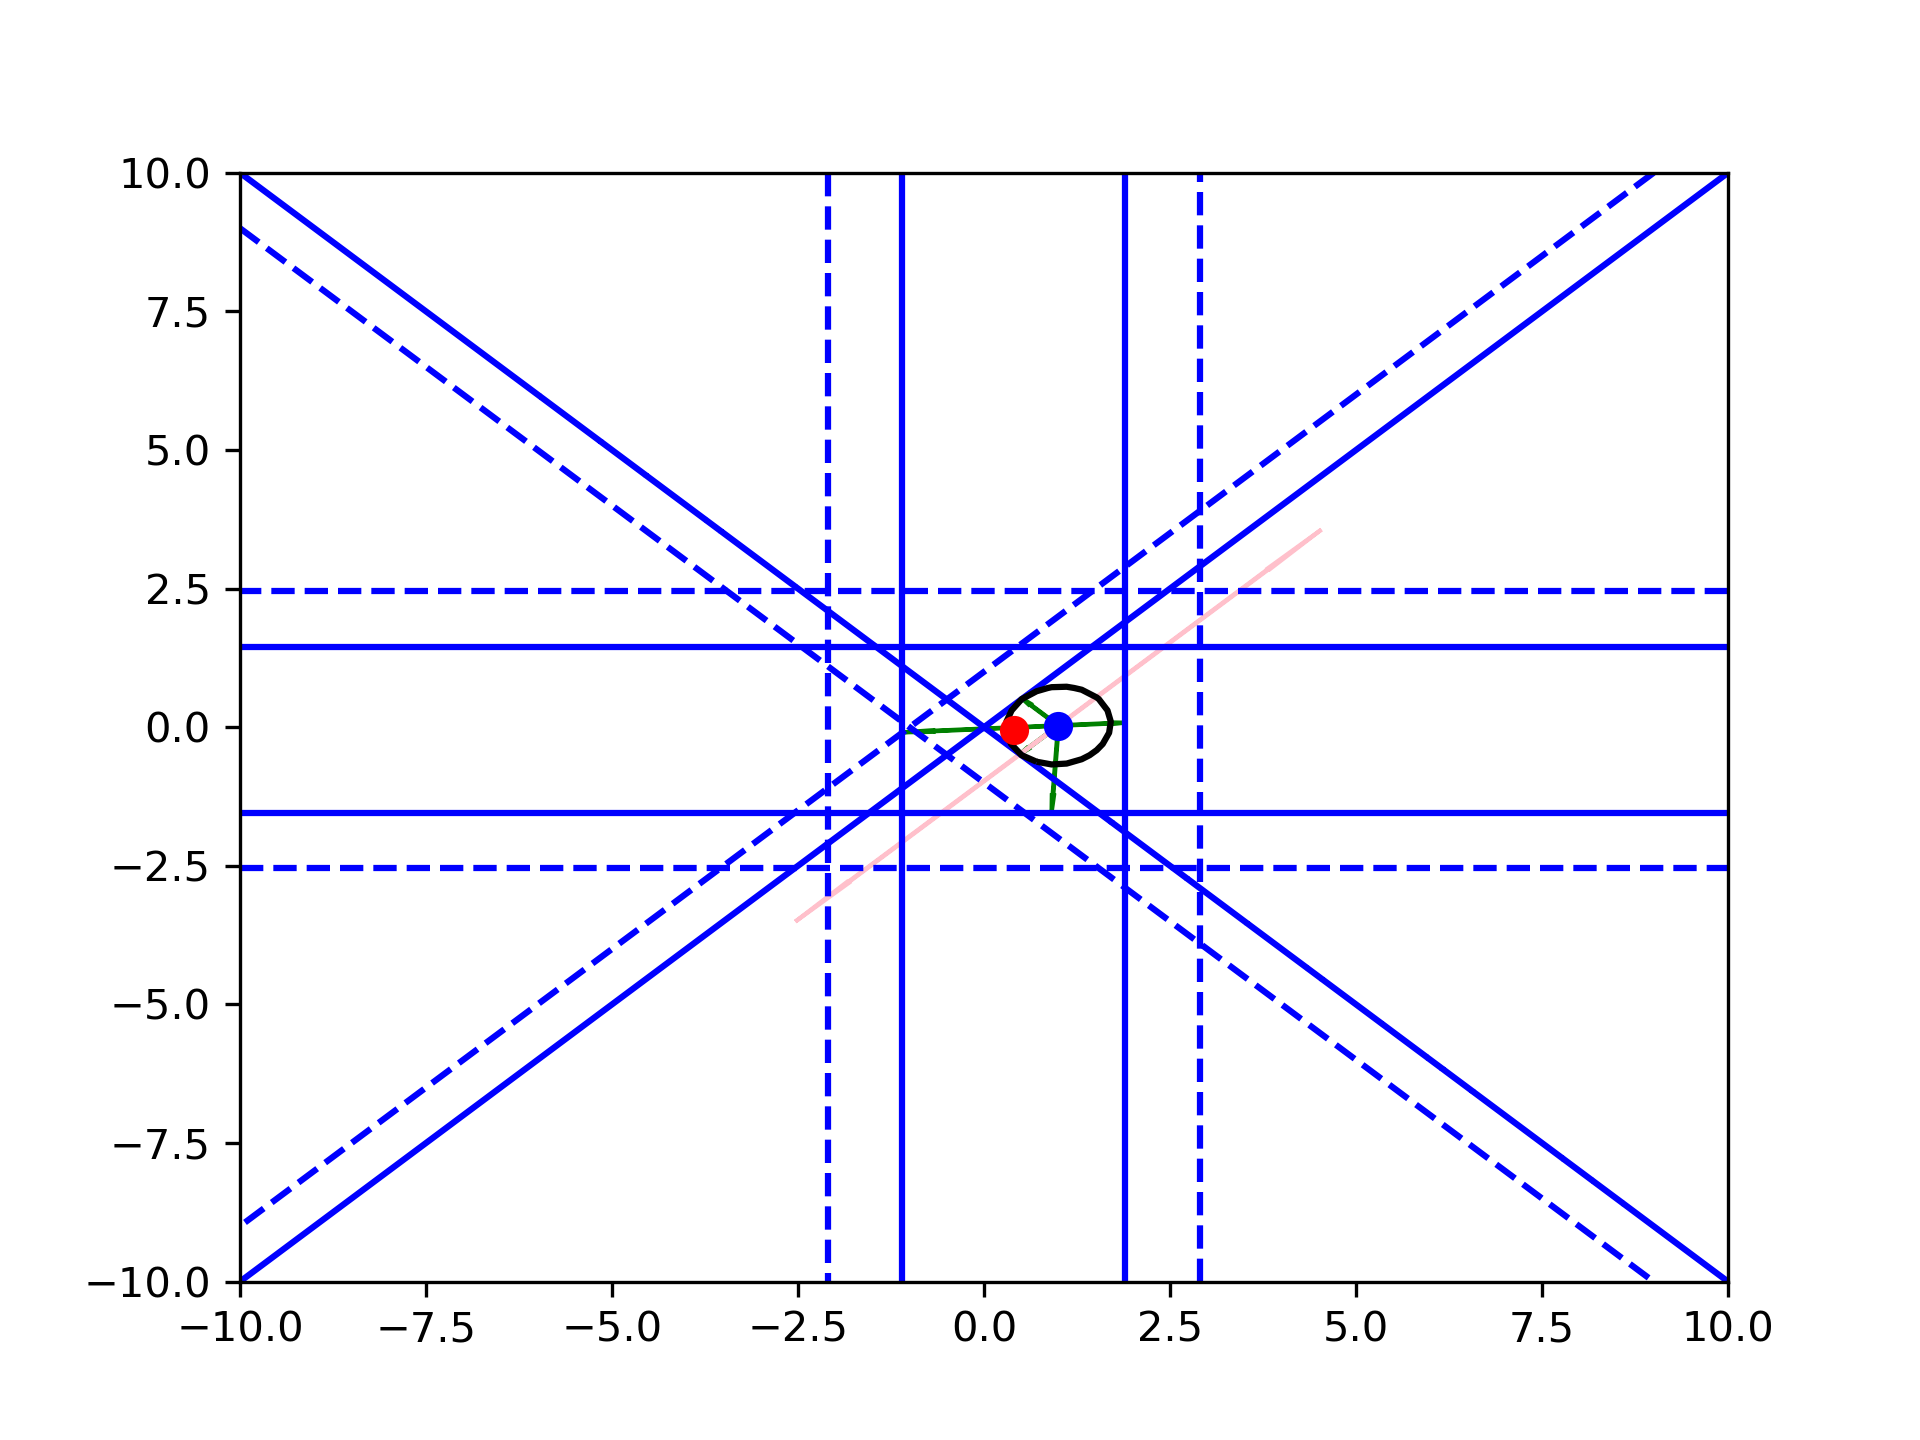
\includegraphics[scale=0.4]{images/everything_runs_2.png}
    \caption[An example of how the search for the sample region center can go wrong.]{
    	An example of how the search for the feasible region center can go wrong.  
     	On the left, a very small sample region is selected; however its proximity to the the minimizer over the outer trust region makes the model more accurate at the minimizer.
    	On the right, a sample region with larger volume is chosen, but it is further from the trust region minimizer.
	}
    \label{ellipse_runs_away}
\end{figure}


\paragraph{Path Searches}

% \sbnote{This discussion is quite vague, and in my opinion, off target.  
% You don't necessarily want to be moving toward a vertex.   
% You just don't want your ellipsoid to move in the opposite direction as  the descent direction.}
% 
% 
% 
% Although $\mfk$'s minimizer over $\outertrk$  can appear anywhere, there are some reasons for expecting it to be at a ``vertex."
% If it lies in the interior, there is little need for using constrained approaches once near the solution.
% 
% 
% %The ellipsoid with maximum volume, however, tends to lead $ \sampletrk $ away from vertices.
% One way of trying to ensure a feasible direction towards a vertex, while still allowing a larger volume ellipsoid, 
% is by limiting the search for the new center to lie on piecewise linear path starting at the current iterate $\xk$.

Rather than searching over all possible center, it may be more efficient to only move away from the boundary.
This can be done using one dimensional search along an appropriate direction.
For example, our first attempt was to simply search a line directed orthogonally away from the closest constraint.
This has obvious problems as shown in \cref{first_line_search}: we should avoid letting the new center get closer to another constraint.    

\sbnote{This could be clearer.   
A key point is that with this method, you can determine the ellipsoid center simply by moving along this line until you are equi-distant from the 2 closest constraints. 
Thus,  there is little gain if the current iterate is close to two or more constraints.}

\begin{figure}[ht]
    \centering
    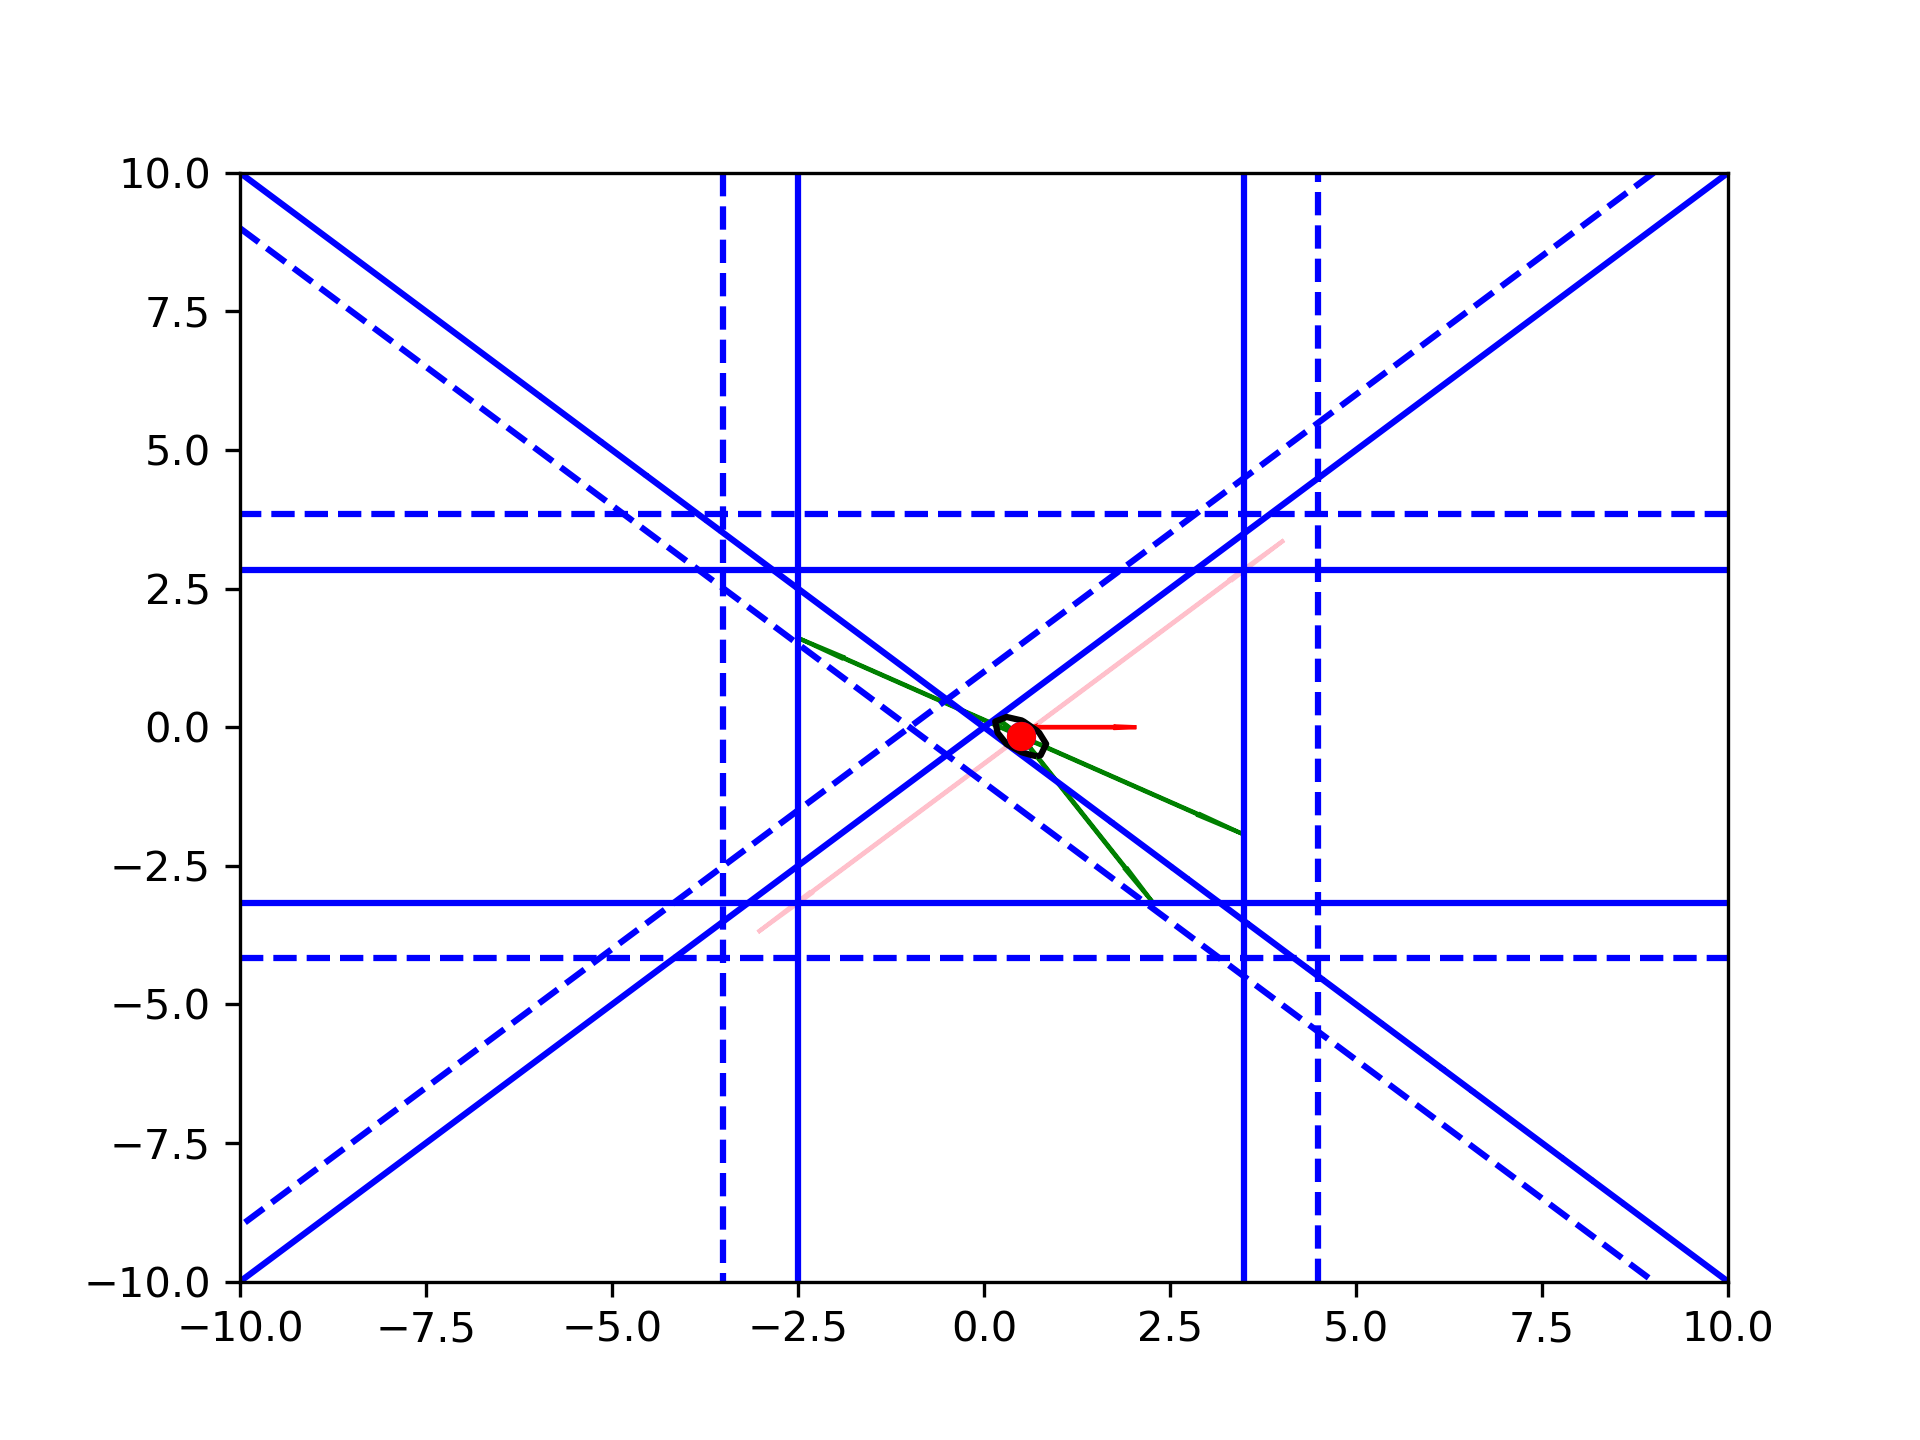
\includegraphics[scale=0.4]{images/line_1.png}
    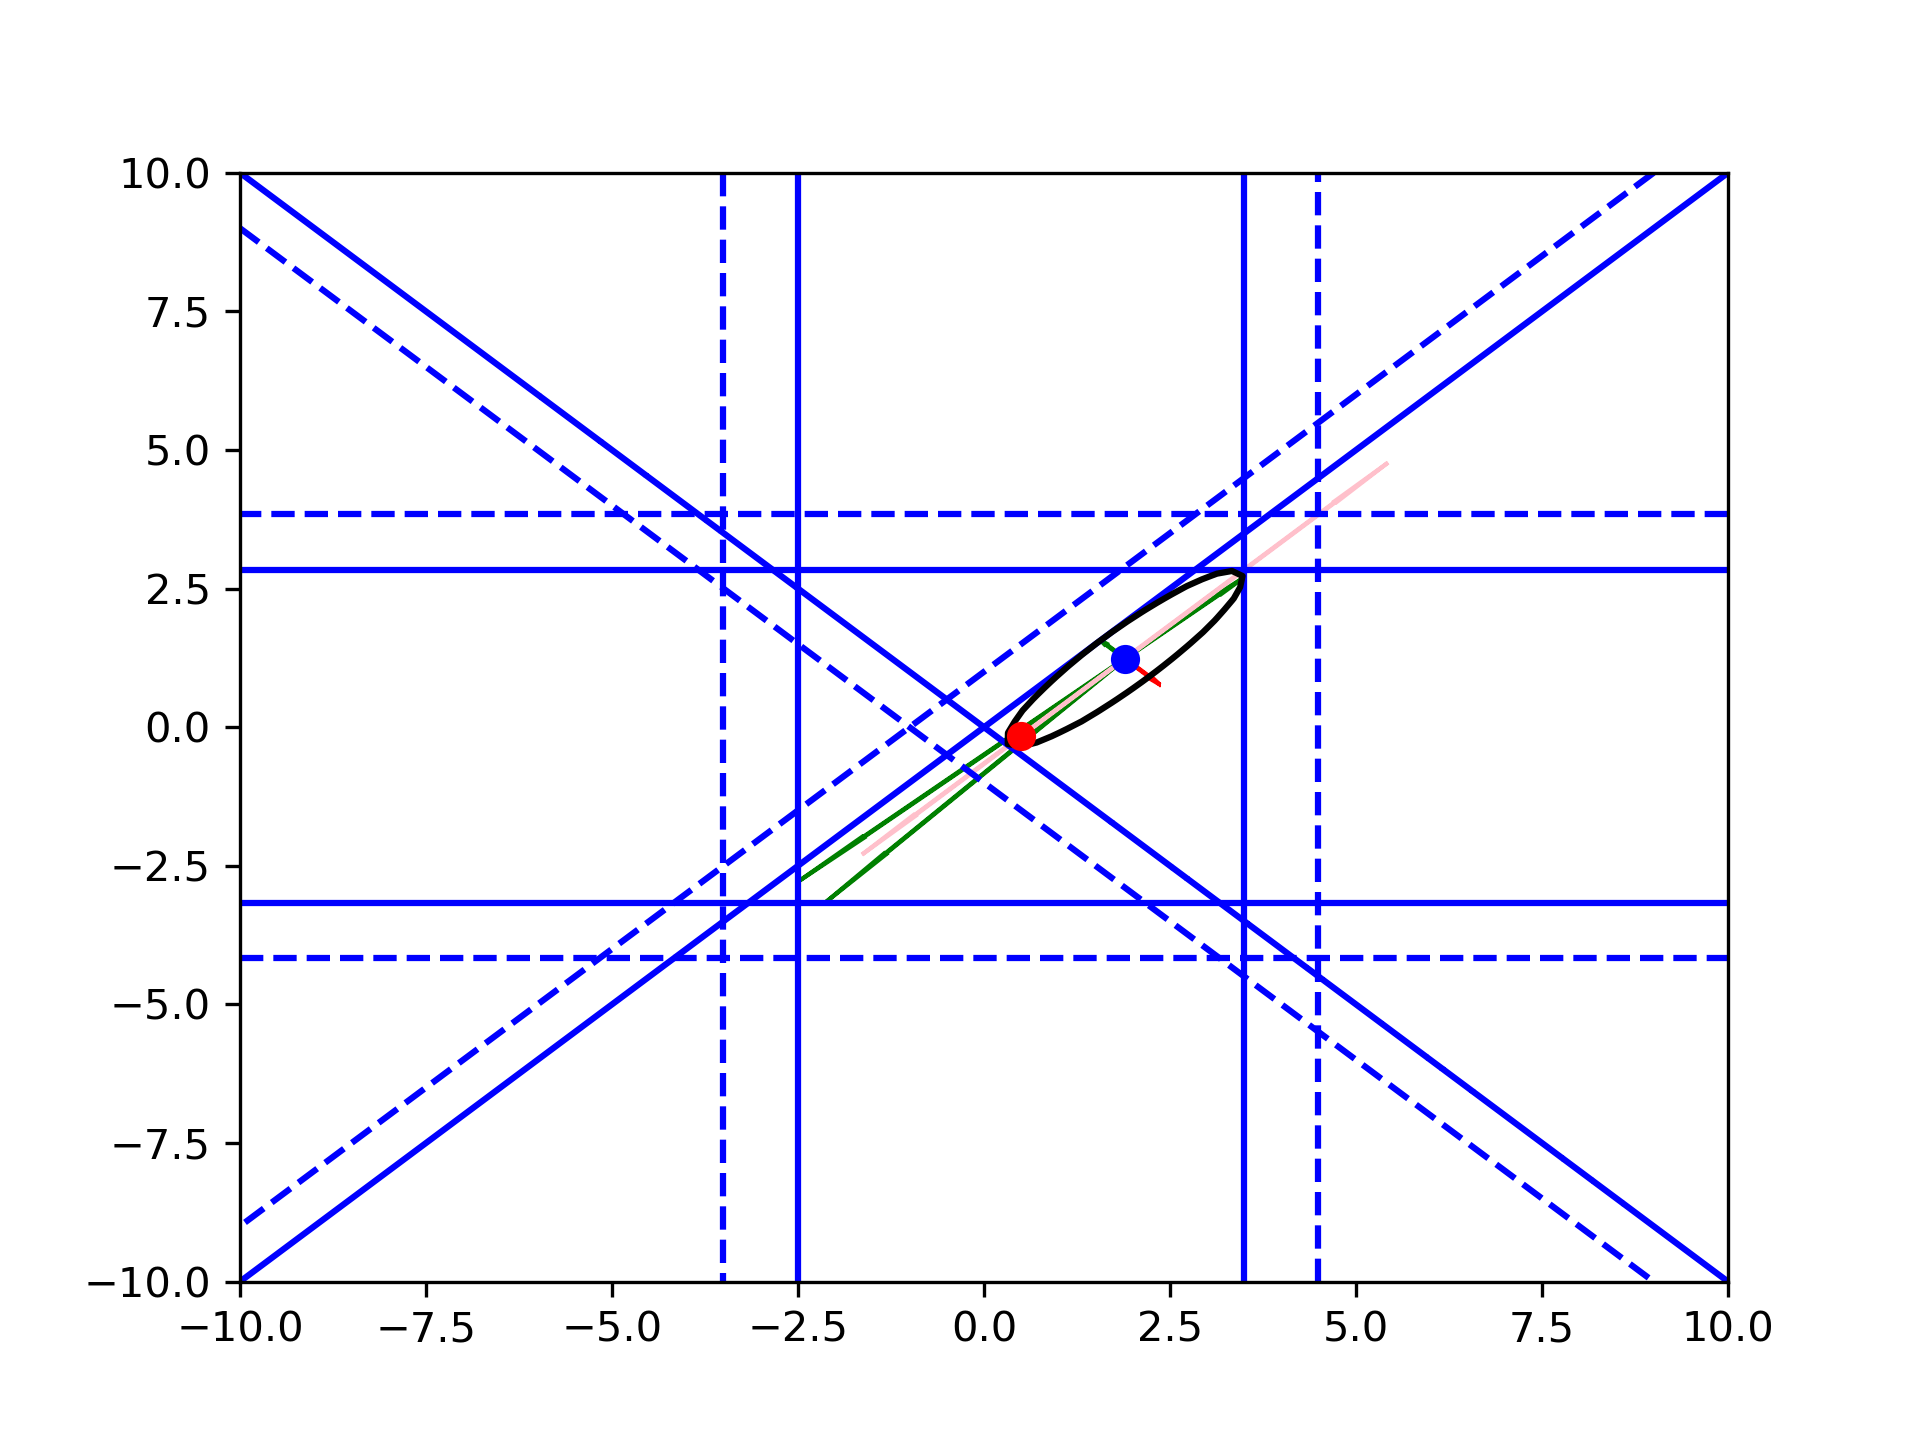
\includegraphics[scale=0.4]{images/line_2.png}
    \caption[Why only considering the nearest constraint is not sufficient. ]
        {Why only considering the nearest constraint is not sufficient.   On the left is the starting ellipsoid.
    	By choosing centers further away from only the nearest constraint, the ellipsoid becomes narrow as another constraint is limiting the length of the second axis.
	}
    \label{first_line_search}
\end{figure}

To fix this, we search along a piecewise linear path leading away from the closest constraints.   
The algorithm works by choosing a set of points $s_0, s_1, s_2, \ldots, s_{n_{\text{points}}}$
that are each equidistant to a subset of the constraint's faces.
The center search then considers points along the line segments between these points.
% Namely, it starts at the current iterate and travels along a ray away from all the closest constraints until it reaches a point equidistant to yet another constraint.

More precisely, the first point is chosen to be the current iterate: $s_0 = \xk$.
The algorithm then repeats the following process for $i$ from $0$ to $n_{\text{points}}-1$.
First, compute the set of nearest constraints, where the distance from the current point the point $s_i$ to each constraint $A_j$: 
is given by $d_j = b - A_j x$.
Recall that the rows of $A$ are normalized: $\left\|A_i\right\| = 1$.
While finding the next point $s_{i+1}$, let  $E$ be the indices of $A$ whose constraints are the equidistant and nearest to $s_i$:
$\{j \in [m] | d_j = \min_{l \in [m]} d_l\}$.
Let the remaining indices be $R = [m] \setminus E$.
The algorithm chooses a search direction $p = {A_E}^Tr$ as a linear combination of the normal vectors of the nearest constraints.
%When the constraint violation of $s_i$ is non-zero, this search ray can be found by finding the point that doubles the current slack ${A_E}s_i-{b_E}$.
%This is given by $r{A_E}^T$ where $r$ solves the linear system ${A_E}(s_i + r{A_E}^T) - b_E = 2 ({A_E}n_i - b_E)$.
%If the current violation is zero, then the right hand side can be set to a vector of all ones to ensure that all slacks violations are the same: $A_E(s_i + r{A_E}^T) - b_E = 1$.
This search ray can be found by setting the slack of each equidistant constraint to twice its current value:
$ b_E - A_E(s_i + {A_E}^Tr) = 2 \left[b_E - A_Es_i\right] \Longrightarrow r = \left[A_E{A_E}^T\right]^{-1}\left(b_E + A_E s_i\right)$.
% $A_E(s_i + r{A_E}^T) - b_E = 1$.
We can travel along this ray until we reach a point that is the same distance to a remaining face.
By travelling a distance $t$, we see that the $j$-th constraint becomes active when
$A_j (s_i + t p) = b_j \Longrightarrow t = \frac{b_j - A_j s_i}{A_jp}$
so that we can travel by 
$t = \argmin_{j \in R} \left\{\frac{b_j - A_j s_i}{A_jp}  \right\}. $
We set $s_{i+1} = s_{i} + t p$.
This process is described in \cref{segment_construction}

Of course, $n_{\text{points}}$ must be less than or equal to $n + 1$ in order for this to be defined.
\begin{boxedcomment}
Also, the algorithm must stop early if $A_E$ contains $n$ parallel normal vectors: 
as there will no longer be a direction that leads away from all constraints.
\end{boxedcomment}


\begin{algorithm}[H]
    \caption{Path segment construction}
    \label{segment_construction}
    \begin{itemize}
        \item[\textbf{Step 0}] \textbf{(Initialization)} \\
            Choose a number of segments $n_{\text{points}} \le n$, and set $s_0 = \xk$, $i=1$.
            
        \item[\textbf{Step 1}] \textbf{(Compute nearest constraints)} \\
			Compute $d_j = b - A_j s_{i-1}$ for each $j \in [m]$, and partition 
			\begin{align*}
			E = \left\{j \in [m] \bigg| d_j = \min_{l \in [m]} d_l\right\}, \; \textrm{and} \; R = [m] \setminus E.
			\end{align*}
			If $|E| \ge n$, then \textbf{Stop}.
			
            
        \item[\textbf{Step 2}] \textbf{(Compute search segment)} \\
        	Compute the search direction $p = {A_E}^T\left[A_E{A_E}^T\right]^{-1}\left(b_E + A_E s_{i-1}\right)$
        	and distance $t = \argmin_{j \in R} \left\{\frac{b_j - A_j s_{i-1}}{A_jp}  \right\}$. \\
        	Set $s_i \gets s_{i-1} + tp$.
        	
        \item[\textbf{Step 4}] \textbf{(Repeat)} \\
        if $i = n_{\text{points}}$ \textbf{stop}, otherwise set $i \gets i+1$ and go to Step 1.
    \end{itemize}
\end{algorithm}


% if we let $\nabla \modelconstrainti\left(\xk\right) = A_i$ be the $i$th row of $A$, then we define the distance from a search point $s$ so the $i$th constraint to be

Once each end point $s_i$ is computed, the algorithm searches along each line segment $[s_{i-1}, s_i]$ for $i \in [n_{\text{points}}]$.
This means that we can define a class of searches that each limit the number of line segments to search $n_{\text{points}}$.
Within the results, these algorithms are described as ``ellipse segment $n_{\text{points}}$''.

In \cref{line_can_run}, the red line shows the line segments equidistant from their closest constraints.
Notice that with two line segments, the algorithm can already choose new centers further from the vertex.

% TODO: REPLACE PICTURES
\begin{figure}[ht]
    \centering
    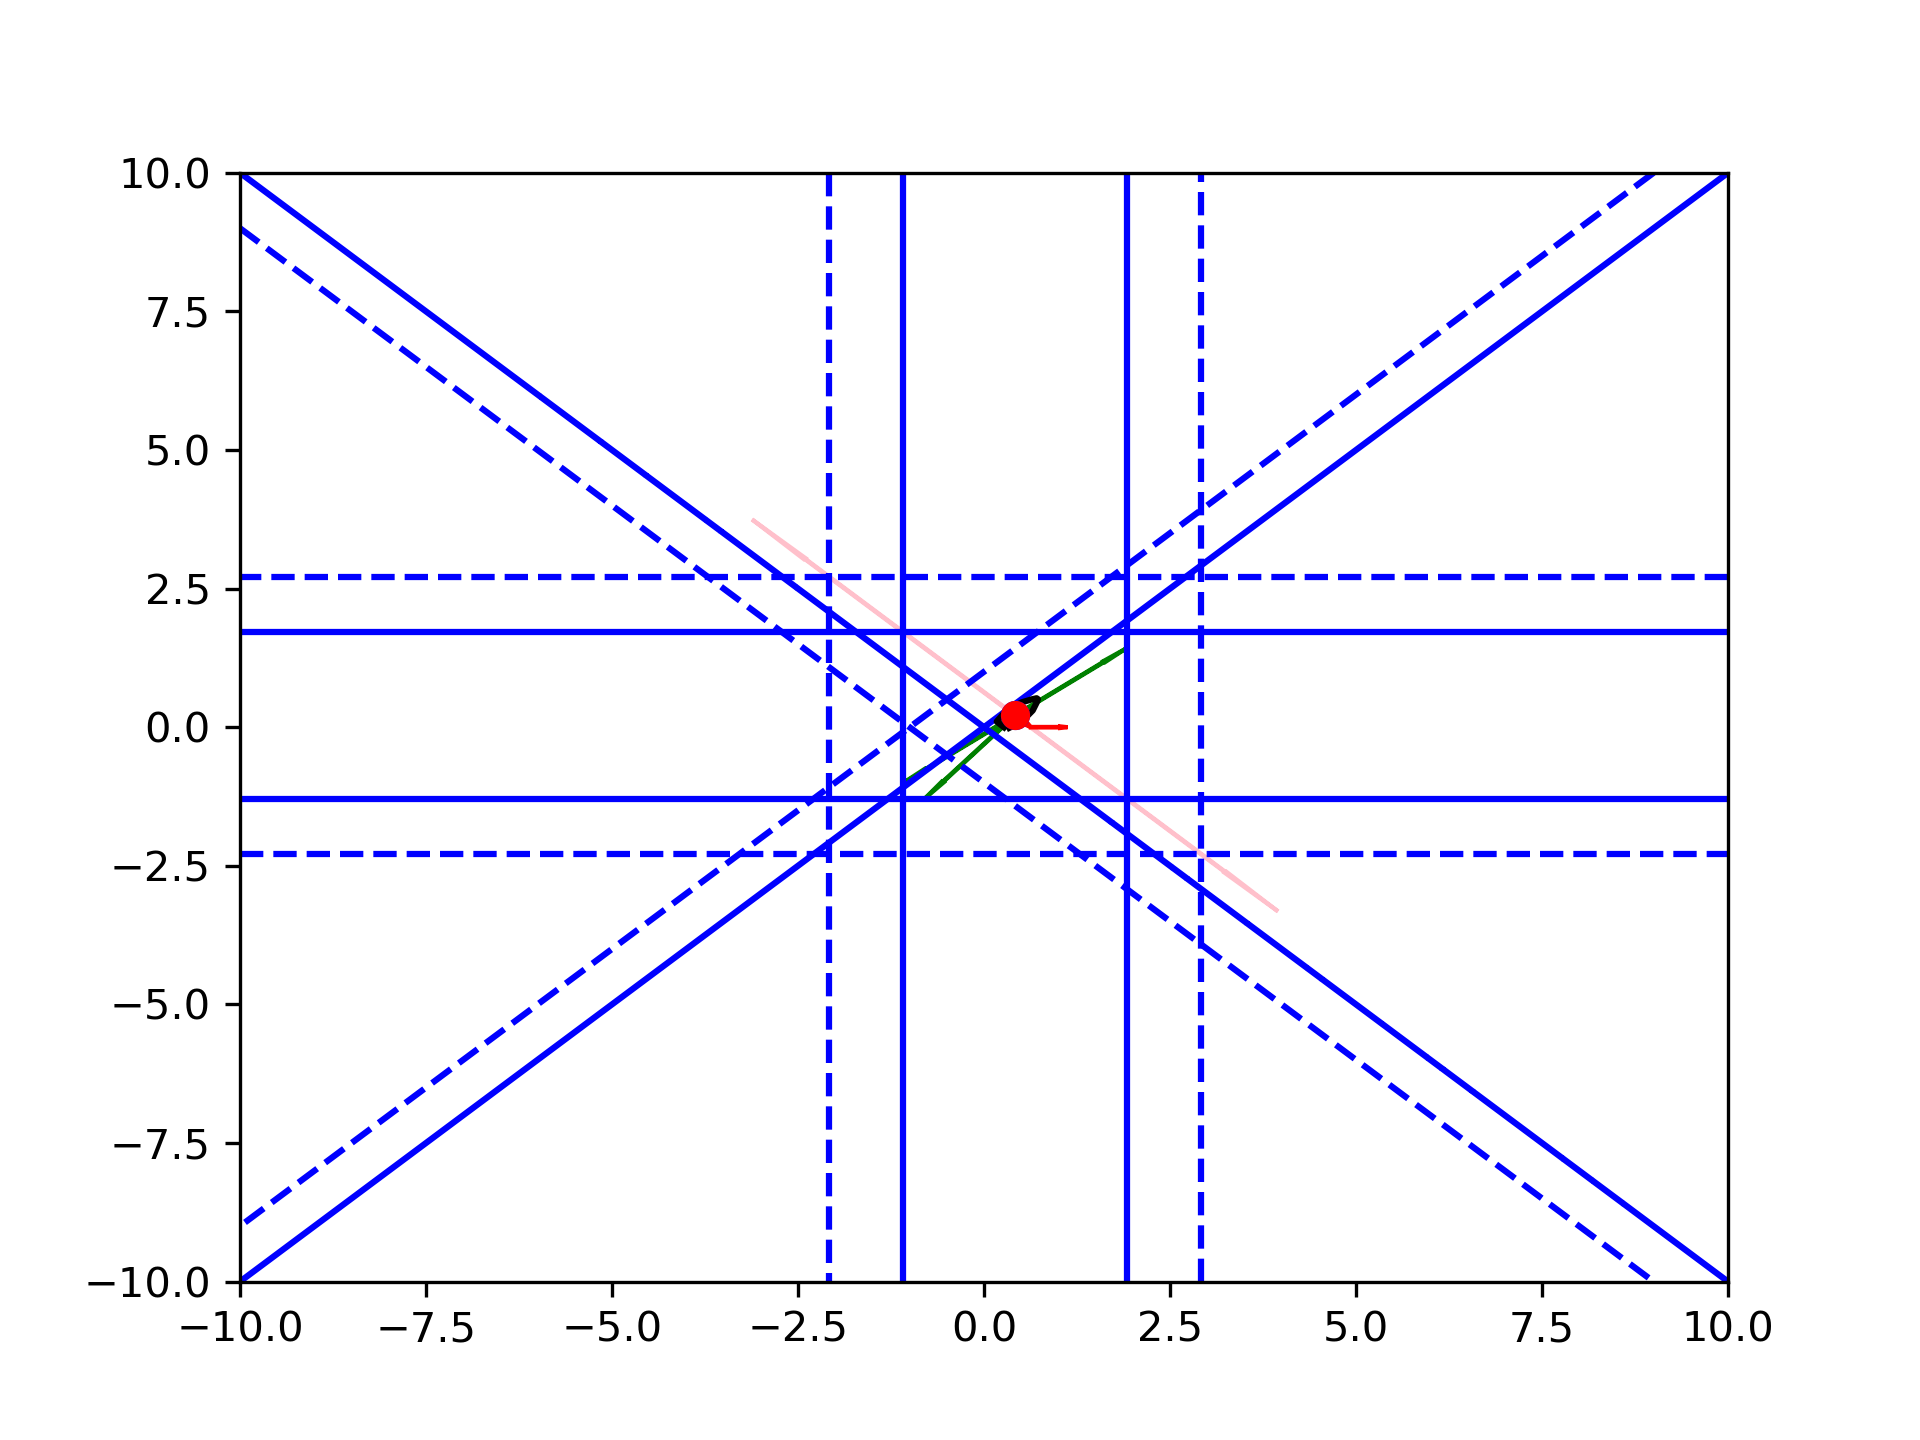
\includegraphics[scale=0.4]{images/run_away_1.png}
    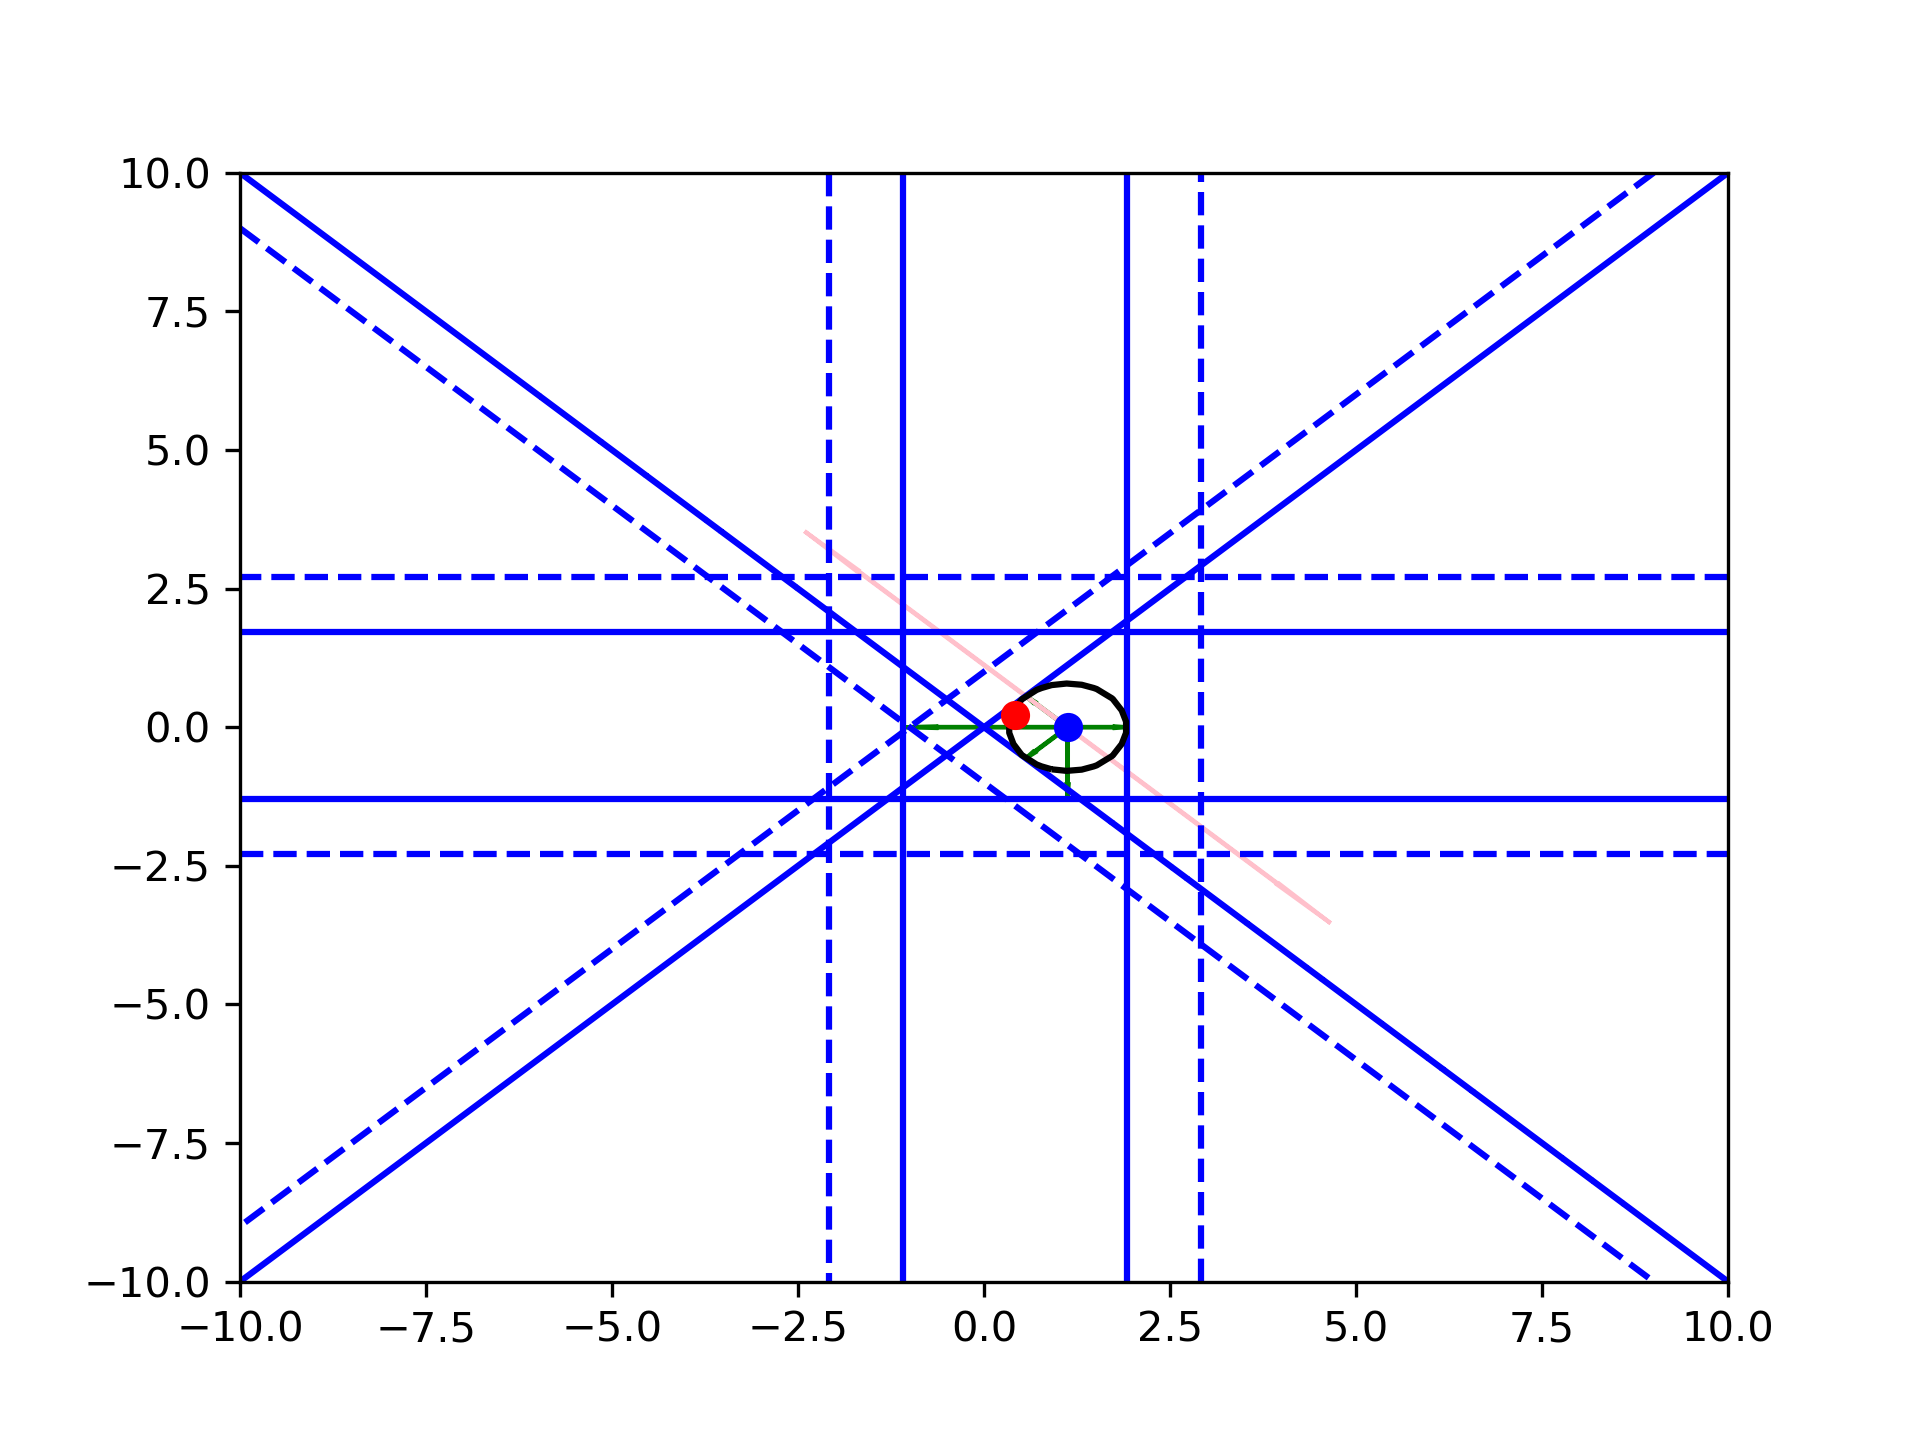
\includegraphics[scale=0.4]{images/run_away_2.png}
    \caption{
%     	\emph{Short:} Why only considering the nearest constraint is not sufficient. 
%     	\emph{Long:} On the left is the starting ellipsoid.
%     	By choosing centers further away from only the nearest constraint, the ellipsoid becomes narrow as another constraint is limiting the length of the second axis.
    Ellipse runs away from the optimizer}
    \label{line_can_run}
\end{figure}


\paragraph*{Circumscribed ellipse}

We also implemented a variant of the algorithm in which the sample region was the smallest volume ellipsoid to contain the feasible region.
Notice that necessarily includes points that are outside the current trust region, and likely infeasible points.
Thus, both the trust region and linear constraints have to be added to the optimization problem defining the replacement point while computing the Lagrange polynomials.
For more details about the this modified model improvement algorithm, see \cref{sec:polyhedral}.

\subsection{Sample Problem}
The first test was on a problem with simple constraints and a pathological objective.
We let $f(x) = \epsilon x + (1-\epsilon)(y - \alpha x \sin(\gamma x))^2$ for a fixed constant $\epsilon$, and set the constraints to be
$x_2 \le ax_1$, $x_2 \ge -ax_1$ for a fixed constant $a$.
We summarize the number of function evaluations and iterations taken within \cref{linear_pathological_results}.

In general, the linear models converge more quickly than quadratic models.
We see that the method with fewest iterations and function evaluations is the linear polyhedral shape.
This is likely due to the fact that the polyhedral shape is allowed to search the entire outer trust region.
This also explains why the circumscribed ellipse and maximum volume simplex also perform well.
%We also notices that with a simple heuristic we were able to improve the ellipse slightly from 170 to 157.
Also, the scaled ellipsoid performs comparably to the unscaled version.

\subsection{Schittkowksi Test Problems}


We tested these algorithms on several problems from the Hot-Schittkowski problem set \cite{Schittkowski:1987:MTE:27135}, \cite{Hock1980}.
We selected the problems that have linear constraints: 21, 24, 25, 35, 36, 44, 45, 76, 224, 231, 232, 250, 251.
We summarize the results within \cref{linear_schittowski_results}.

% 37 was left out because it proved to be difficult.

\paragraph*{Performance Profile}
\label{performance_profile}
In order to better evaluate the algorithms on the problems across in this test set, we use a performance profile developed in \cite{More:2009:BDO:1654367.1654371}.
Given a set of Solvers $\mathcal S$ that solved a set of problems $\mathcal P$ with the number of evaluations of solver $s$ on problem $p$ being $N(s, p)$, the performance ratio is defined to be $r(s, p) = \frac{N(s, p)}{\min_{s \in \mathcal S} N(s, p)}$.
If the algorithm does not complete, then the number of evaluations is set to $\infty$.
The performance profile of a solver $s$ and parameter $\alpha \in [0, \infty)$ is then the number of problems for which the performance ratio is less than or equal to $\alpha$: 

\begin{align}
\rho(s, \alpha) = \frac 1 {\left\|\mathcal P \right\|} \left\|p \in \mathcal P | r(s, p) \le \alpha\right\|.
\end{align}

The $y$ axis of a performance plot is the performance profile, and the $x$ axis is the parameter $\alpha$.
Note that algorithms with high performance profiles for small values of $\alpha$ solved a large number of problems the most with the fewest evaluations, while algorithms that eventually reach high performance profiles with larger values of $\alpha$ solve a large set of problems.
The performance profile for the Hot-Schittkowski problem set is give in figure \cref{performance_profile_image}.


\begin{figure}[ht]
    \centering
    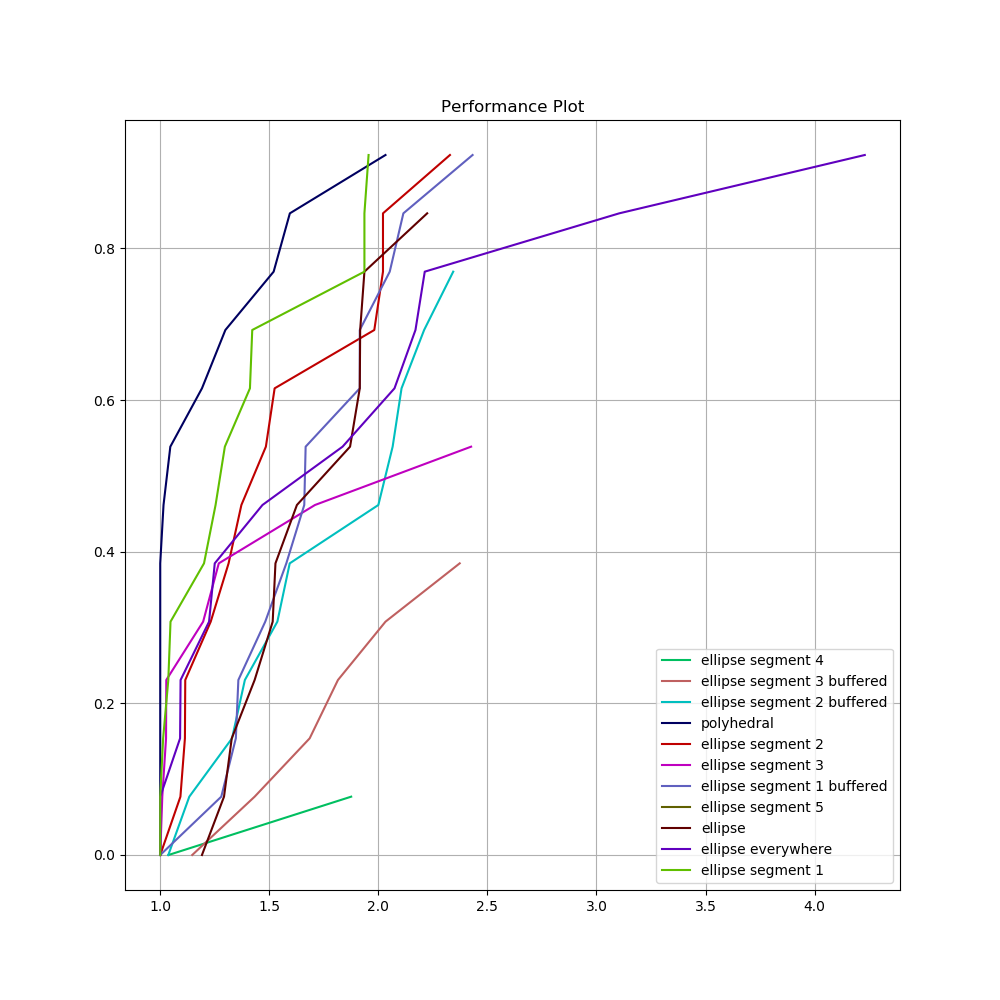
\includegraphics[scale=0.4]{images/performance_profile_plot.png}
    \caption[A performance profile comparing different variants of the algorithm for linear constraints.]{
    	A performance profile comparing different variants of the algorithm for linear constraints.
    	We see that the polyhedral algorithm is both efficient and robust.
    }
    \label{performance_profile_image}
\end{figure}



The line segment search with 5 segments does not solve many problems, this is because several of the problems have dimension less than $5$, so that it was not even ran on these.
Notice that the polyhedral search does very well.
We conjecture that this may not hold with modelled, nonlinear constraints.


\subsection{Summary}
We still experienced a problem with iterates coming too close to the boundary of the feasible region.
Another way of dealing with this is to shift the constraints closer to the current iterate.
Namely, we introduce a parameter $\upsilon$ to determine how far to scale the constraints.
Then, within the trust region subproblem, we add constraints of $Ax \le b\upsilon + (1-\upsilon) A \xk $.
Before doing this, the rows of $A$ are normalized.
This produces the buffered segment searches withing the results.

% \color{red}
% 
% \section{Figure out where goes}
% 
% From here on, we will assume that the iterates $\xk$ are chosen according to \cref{linearly_constrained_dfo}.
% This implies that each of the sample points used to construct $\mfk$ are output of \cref{model_improving_algorithm}.
% 
% Because \cref{lipschitz_gradient} and \cref{lipschitz_hessian} are satisfied, $f$ also satisfies \cref{introduction_3_1} and hence the assumptions for \cref{quadratic_errors}.
% Notice that because $\kappa_f$, $\kappa_g$, $\kappa_h$ only depend on $p$, $L_h$, and $\Lambda$, these values do not depend on the iteration $k$:
% using the same tolerance $\xi_{\text{min}}$ within \cref{model_improving_algorithm} implies a bound on $\Lambda$.
% , and therefore $\mfk$ satisfies the requirements for \cref{quadratic_errors}.
% is a fully quadratic model over $B_{\infty}(\xk, \dk)$.
% \color{black}

